\documentclass[a4paper, 12pt]{article}

\usepackage[a4paper, inner=1.7cm, outer=2.7cm, top=2cm, bottom=2cm, bindingoffset=1.2cm]{geometry}
\usepackage[english]{babel}
\usepackage{graphicx}
	\graphicspath{ {images/} }
\usepackage{wrapfig}
\usepackage{paralist}
\usepackage{blindtext}
\usepackage{enumitem}
\usepackage{fancyhdr}
\usepackage{amsmath}
\usepackage[utf8]{inputenc}
\usepackage[toc,section=section]{glossaries}
\usepackage{enumitem}
\usepackage{float}
\usepackage{listings}


\makenoidxglossaries
 
\newglossaryentry{java}
{
    name=Java,
    description={A general purpose object-oriented programming language}
}

\newglossaryentry{javafx}
{
    name=JavaFX,
    description={A graphical user interface library for Java}
}

\newglossaryentry{git}
{
    name=Git,
    description={An open sourece distributed version control software}
}

\newglossaryentry{github}
{
    name=GitHub,
    description={A web service that hosts git repositories for ease of use between developers}
}

\newglossaryentry{discord}
{
    name=Discord,
    description={A communication software hosted on the web used for scheduling, discussion and sharing of files}
}

\newglossaryentry{junit}
{
    name=Junit,
    description={A library in Java used for writing unit tests}
}

\newglossaryentry{latex}
{
    name=Latex,
    description={A textual interface for writing technical and scientific documents}
}

\newglossaryentry{javadoc}
{
    name=JavaDoc,
    description={A code documentation generator for Java}
}

\newglossaryentry{transcendentalfunction}
{
    name=Transcendental Function,
    description={"A function that does not satisfy any single-variable
polynomial equation whose coefficients are themselves roots of polynomials"}
}

\newglossaryentry{eclipse}
{
    name=Eclipse,
    description={A Java Integrated Development Environment}
}

\newglossaryentry{intellij}
{
    name=IntelliJ,
    description={A Java Integrated Development Environment}
}


\makeindex

\setlength{\parindent}{0pt}

\begin{document}


% TITLE PAGE CODE ------------------------------------
\title{\LARGE{\textbf{Team F - ETERNITY Calculator}}}
\author{
	Castonguay, Justin | Fakhr, Daniel | Hernandez, Jaime Andres \\ Thibault-Shea, Daniel |
	Yaghma, Ashkhan \\
}
\date{August 5, 2019}

\fancyhf{}

\clearpage\maketitle
\thispagestyle{empty} % Ensures no page numbering on title page
\pagebreak

\setcounter{page}{2} % Start counting on page 2
\fancyhf{}
\renewcommand{\headrulewidth}{2pt}
\renewcommand{\footrulewidth}{1pt}
\fancyhead[LE,RO]{\rightmark}
\tableofcontents
\pagebreak


\section{Introduction and Lead Up to Iteration 2}

\subsection{Recap of Iteration 1}

During iteration 1 we focused on the overall setup of our team and project before moving forward with any implementation. For starters we set up clear expectations of how we expected to work together to encourage efficient and collaborative team dynamics amongst each other. We also set up a clear strategy that involved distributing the workload while being conscious of each other's skill sets. Regarding the strategy, we also had to agree on what technologies we would use and how we would test our code in order to approach the implementation together in an efficient manner and meet our deadlines successfully. 
\\

Before having to start on the implementation we also interviewed individuals with different technical backgrounds to gather information of what their needs were for their ideal calculator and how we could cater to those needs. From this we built a list of personas where we were able to group specific people from the interviewees in general categories to better understand what they all wanted in a more abstract way. The 3 personas we created consisted of a technical/mathematical, common/casual, and an Academic persona. We then used these findings in order to build use cases to obtain a more concrete idea of how our implementation would function before creating them. Finally, we began to work on our respective responsibilities and the Engineering of our project. 

\subsection{Intro to current Iteration}

For this iteration, our main focus has been mainly about the implementation of the Calculator itself. In other words, we could say this is the Engineering stage while in the beginning stages we were more focused on preparation and gathering of data to back up our reasoning of why we should implement something the way we decided to. 
\\

This new iteration involved some important steps worth mentioning. One important aspect we focused on was making sense of the data and beginning to make clear decisions on how to apply it to our project. Also during the process where each function was being implemented, each one of us had to find different methodologies to actually make the functions work. For example, there could’ve been different ways to implement the Sin(x) function in Java, but we had to find one that would get us the closest to an accurate and precise result, while also having it run and execute successfully! To do this we each had to identify what were the possible solutions or concepts we wanted to implement, weigh out the pros and cons of each, choose one, and then execute it. Many times this involved looking up mathematical formulas online or within textbooks. We have documented this process throughout this report. 
\\

In addition to the function of the calculator, the UI was another main focus throughout this iteration. As we have learned during class, the UI is a very important aspect that allows the user to understand how the software works and it facilitates the process of understanding how to use the software, if properly designed of course. As the GUI was being made our group actively provided feedback to improve our GUI experience while saving us time before reaching a final product/concept. 
\\

Lastly, aside from the functions, we also realized we needed to dedicate time to creating a validator and parser to successfully pass through the mathematical expressions to successfully solve them with the operations and functions we created. This was one of the most tedious but most important things to focus on throughout this iteration. 
\\

Other aspects that weren’t as time consuming as the tasks previously mentioned but still important was implementing error messaging, continuing to review each other's work to encourage efficient synergy, resolving any remaining edge cases for our functions, and checking in with individuals we interviewed to review if what we created met their expectations to find out what improvements would have to be made in the future. 




\subsection{Goals for current Iteration}

To summarize, the main goals we set out to complete during this iteration were the following:
\\

\begin{compactitem}
\item Parser creation
\item Validator creation
\item Implementation selection for functions
\item GUI implementation
\item Quality Assurance (i.e. Teammate/peer code Review)
\item Error message creation
\item Resolving edge cases
\end{compactitem}

\section{Team organization and collaboration patterns}

\subsection{Expectations}

The first thing on our order of business was to do a round table discussions to get everyone's expectations with regards to the team dynamics. The reason for this was so that we would all be on the same page.

\medskip

\textbf{Danny:}
\begin{compactitem}
\item Do mathematical research before coding any mathematical functions.
\item Be able to code in java and have decent technical knowledge 
\item Be willing to compromise ,or put matters to a vote, at times of conflict
\end{compactitem}
\textbf{Dan: }
\begin{compactitem}
\item The team should be a supportive place where member can develop - if someone doesn’t know something then the team should be able to teach them. We need to communicate actively and keep our peers in the loop.
\end{compactitem}
\textbf{Justin:}
\begin{compactitem}
\item I expect everyone to respect each other and have realistic expectations of one and other.
\item Everyone listen to each other and learn from each other.
\end{compactitem}
\textbf{Ashkan:}
\begin{compactitem}
\item It seems my level of knowledge is lower than the average of team. So I expect the team to bear with me, assign some simpler tasks to me in the beginning and support me to catch up as soon as possible.
\end{compactitem}
\textbf{Andres:}
\begin{compactitem}
\item I expect everyone to be respectful with each other
\item I expect everyone to communicate with each other openly
\item I expect everyone to be able to communicate if they will not be able to finish a part on time in a timely manner, so adjustments can be made before the deadline with minimal stress
\item I expect the work to be spread fairly
\item I expect the work to be spread out considering everyone’s skill sets and what they would like to work on themselves
\end{compactitem}

\textbf{Expectations Agreed on:}
\begin{compactitem}
\item The team should be a supportive place where member can develop - if someone doesn’t know something then the team should be able to teach them. We need to communicate actively and keep our peers in the loop.
\item Respect one another
vLearn from each other
\item Listen 
\item Communicate openly and constructively
\item All tasks must be completed before the given deadline
\item If work will not be finished it MUST be communicated in a timely manner so the team can support and readjust our strategy to deliver our work on time
\item Team outings after milestones on a budget
\item Distribute work fairly, evenly, and considering each member’s skill level.
\end{compactitem}
\bigskip

This document hereby confirms that all group members listed agree to follow through with these expectations throughout the timespan of this whole project. 


\begin{center}
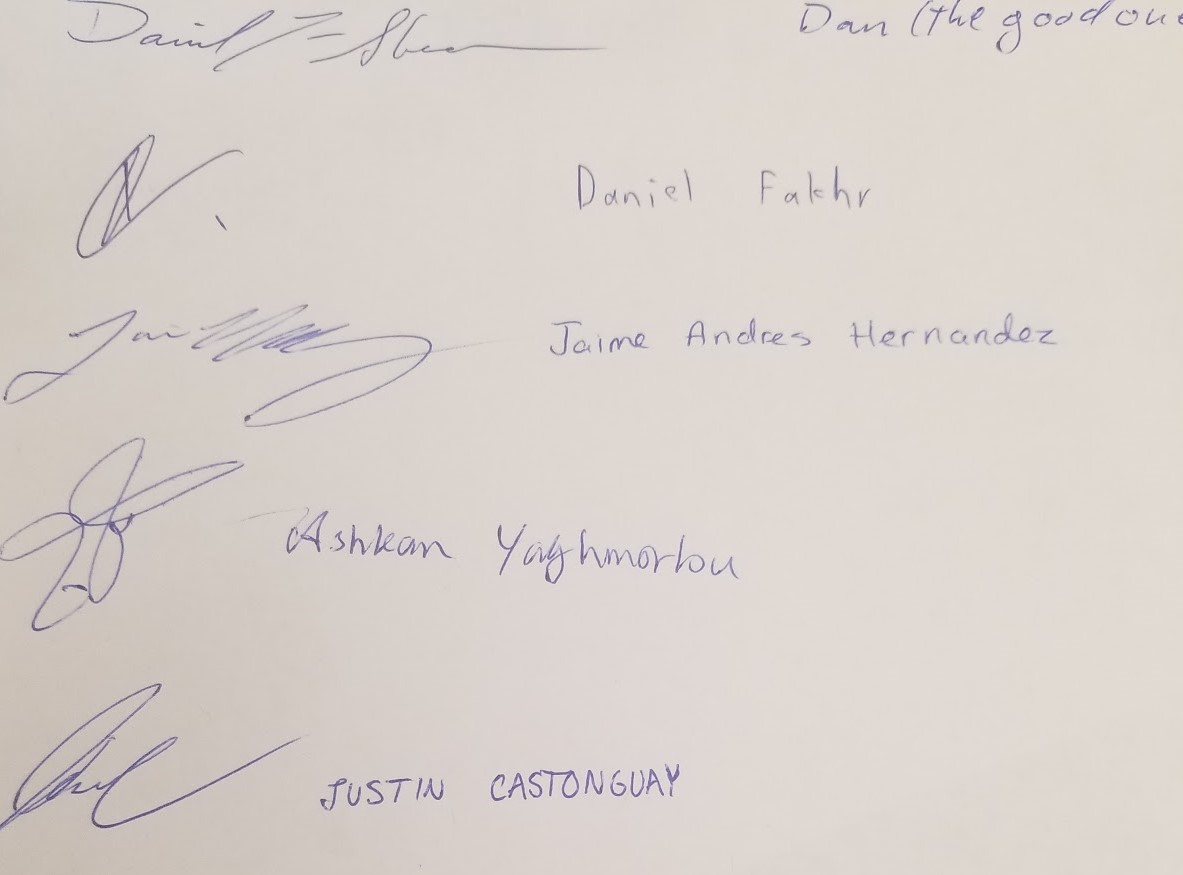
\includegraphics[width=0.4\textwidth]{ExpectationSignatures.jpg}
\end{center}

\subsection{Meeting Schedule}

We agreed to meet at least once a week for 2 hours. We are also in constant contact on Discord and we all keep apprised of recent pushes to the Git repository to stay up to date with the advancement of the code base and the accompanying documents. Detailed meeting minutes are posted to the Git repository after every meeting by the designated secretary for that meeting. We are also using Google Docs to collaboratively work on draft documentation, which can then be used to create our final documentation with the correct formatting.

\subsection{Our Strategy}

In order to develop a working software calculator prototype in the coming weeks, our team has come up with a development strategy to be prepared for challenges that we may face. This strategy must take into account a plan for writing requirements for features implemented, the technologies selected to develop the calculator, ideas of algorithms for numerical computation of selected functions, and tasks to be allocated to each team member based each of our strengths. With a well advised plan of action, we are much more likely to collaborate efficiently as a team and ultimately meet the deadline of the project. 

\subsection{Choice of technology}

Our team needed to select technologies to meet our software needs while also complementing the team members’ development expertise. The necessary technologies included:
\medskip
\begin{compactitem}
\item main programming language with unit testing libraries, a code documentation interface and a graphical user interface library
\item communication tools
\item version control software
\end{compactitem}
\medskip
For our primary programming language we decided to pick the language in which all of our team members had experience writing code in, Java. This allowed each team member to jump right into coding when the time came since no one was blocked having to learn a new language. Java is also advantageous since it has many libraries that we would be able to use for unit testing (Junit), GUI development (JavaFX) and code documentation (Javadoc). Additionally, its object-oriented design fit with how we envisioned designing our calculator program. \\

In order to coordinate with each other outside of regular meeting hours, we decided to use Discord as our communication tool. Discord can be accessed on almost any device, is very reliable and is easy to use. It also allowed us to create different chat channels for different subjects in order to keep our discussions on topic. For example, one channel could be for scheduling and one could be for brainstorming ideas about algorithms. \\

We decided to choose git as our version control software since it is simple enough to use, it has tons of documentation to support our needs and some of our team had already used it. Furthermore, they would allow us to work on the same files at different times and easily keep track of changes made to any of the files. 

\subsection{Task assignment}

During the second team meeting we went over the requirements for deliverable 1 and made a list of all of the things that needed to get done. We quickly saw that this was a significant amount of work and that there were some dependencies between the tasks (ex. do interviews before use cases). We divided the tasks into 3 categories: 1) Information gathering, 2) Consolidation/Report, 3) Coding and prototyping. A cursory evaluation of the workload vs. the deadline showed that we could not possibly deliver all of these tasks on time. Rather than cut out the early-stage prototyping entirely, we decided on making a priority matrix of our tasks with the simple rule that higher priority tasks should be completed before an individual started work on the lower priority ones. \\

We reasoned that the top priority items were those on the critical path of deliverable 1. We all had a good idea of what a calculator should be but we also knew better than to make a product for the developers. Consequently, we absolutely needed the information from the interviews as soon as possible so that we could align our efforts with what the calculator's potential users wanted. This step was so critical and urgent that we put 4 people on it with highest priority. \\

We then consolidated and paraphrased the interview data. We were surprised at just how much information we got from 5 interviewees. Firstly, we extracted the key features each user wanted. Secondly, we distilled down each interview into the key themes that were important for that interviewee. Thirdly, we were able to classify our interviewees based on their expected usage of the calculator (basic use, mathematical use). Lastly, we looked for commonality across the different wants of the interviewees and obtained what we think is a much better approximation of what the market wants from a calculator. \\

One team member was tasked with coming up with an outline of our testing strategy. We decided that since the users all seemed to value accuracy of the mathematical function on the calculator then a test-driven approach to development would be appropriated. \\

Another person was tasked with researching the algorithms needed for the implementation of the non-trivial calculator functions. Some functions had multiple algorithms that varied in complexity. For this first iteration, it was decided that simplicity should be the key criteria in the choice of algorithm since the deadline was so tight. We all agreed that we could reevaluate this strategy for the next iteration. \\

The very last priority was the implementation of the mathematical functions. Some team members were eager to start coding but we decided that it would be a much better idea to focus on the requirements gathering at this stage of development. Consequently, only a very rough implementation of some of these functions appear as code. \\

\begin{table}[ht]
\centering
\caption{Task Priority Matrix}
\begin{tabular}{|l|l|l|l|}
\hline
\textbf{Name}&\textbf{Priority 1}  &\textbf{Priority 2}  &\textbf{Priority 3}  \\ \hline
 Ashkhan&SE Artifacts  &Macro architecture  &$a^x$, $10^x$  \\ \hline
 Daniel F.&Parser  &Newtonian algorithm  &$x^y$,   \\ \hline
 Daniel T.&Validator  &Micro architecture  &$e^x$  \\ \hline
 Jaime&SE Artifacts  &Macro architecture  &$cos(x)$, $sin(x)$  \\ \hline
 Justin&GUI  &Micro architecture  &$ln(x)$  \\ \hline
\end{tabular}
\end{table}

\subsection{Testing strategy}

For testing purposes, we decided to use Junit to write all of our unit tests. These tests would verify the functionality of our different mathematical functions. We would need to think of and write up as many test cases as possible for different scenarios (negative numbers, large and small numbers, invalid input, etc) in order to cover all potential issues. \\

Test coverage is incredibly important in the early stages of a software project. Early and thorough testing reduces the risk of having an insurmountable amount of bugs later on. Taking this into consideration, we decided to employ a Test Driven Development strategy in which we would write unit tests before the functions were complete and imposed a rule that all valid tests must pass before any team member makes a push to our master branch. This would ensure that whenever anyone pulled from the master branch, they would not have to waste time fixing someone's bugs to work on their own task. \\

We all agree that testing each other's code is of paramount importance to the project. To not do so would lead to colossal wastes of time in tracking down myriad bugs. We made the following testing matrix which will ensure that there are no conflicts of interest in the testing. The arrow indicates who can test who - no arrow means you cannot test that person's code.

\begin{figure}[!h]
\caption{Testing matrix}
\centering
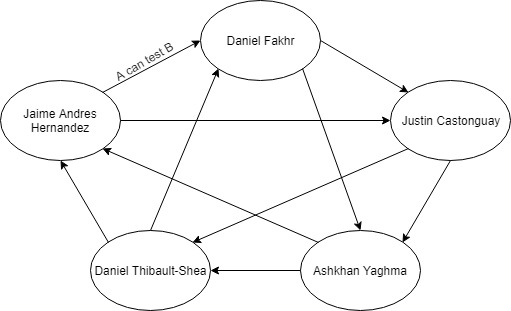
\includegraphics[width=0.75\textwidth]{TestingMatrix}
\end{figure}

The source code peer review was organized such a way that no pair of people review each others code. \\

The code review was done in the similar order :

\medskip
\textit{Jaime Andres Hernandez $\rightarrow$ Daniel Fakhr $\rightarrow$ Justin Castonguay $\rightarrow$ Ashkan Yaghma $\rightarrow$ Daniel Thibult-Shea $\rightarrow$ Jaime andres Hernandez.}
\medskip

The following table summarize some of the code reviews that were undertaken and the associated comments provided to the reviewees.


\begin{table}[]
\begin{tabular}{|l|l|l|}
\hline
Reviewer                                                            & Reviewee                                                         & Comments                                                                                                                                                                                                                                                                    \\ \hline
\begin{tabular}[c]{@{}l@{}} Andres Hernandez\end{tabular} & Daniel Fakhr                                                     & \begin{tabular}[c]{@{}l@{}}-Some functions break for edge cases\\ -Use spacing in math expressions\end{tabular}                                \\ \hline
Daniel Fakhr                                                        & Justing Castonguay                                               & \begin{tabular}[c]{@{}l@{}}-Try to make shorter functions\\ -Use K\&R formating (check online) \\ -Stick to java conventions in mathematical \\ expressions\end{tabular} \\ \hline
Justin Castonguay                                                  & Ashkan Yaghma                                                    & \begin{tabular}[c]{@{}l@{}}-Use more detailed comments\\ -Use better variable names\end{tabular}                                                                                                                                                                               \\ \hline
Ashkan Yaghma                                                       & Daniel Thibault-Shea                                             & \begin{tabular}[c]{@{}l@{}}-Don't leave commented code.\\ -Comment your functions.\end{tabular}                                                                                                                                                                             \\ \hline
Daniel Thibault-Shea                                                & \begin{tabular}[c]{@{}l@{}}Jaime\\ Andres Hernandez\end{tabular} & \begin{tabular}[c]{@{}l@{}}-Comment on what a function does rather than \\ what a function is\\ -Try to shorten your comments while\\  maintaining clarity\end{tabular}                                                                                              \\ \hline
\end{tabular}
\end{table}

\pagebreak


\section{Interviews of Potential Users}

In order to create software requirements, our team got together to brainstorm ideas for what features the calculator would have and how to implement them. We made sure our features were realistic, keeping in mind the time constraint of the project and the development experience of the team. Once we had a base for how we thought our calculator could be developed, we decided to conduct interviews on potential users to find out what features everyday users of calculators actually valued and if our initial ideas complemented these. \\

From the answers from our interviewees, we created user personas that had concrete problems and tasks that needed to be completed and that our software would solve. The user personas along with our initial discussions would then inform what different use cases might be for our calculator. The use cases were put into a standard use case diagram so that the high-level design of the calculator could be understood at a glance. Each use case was then expanded in a summary use case description.
\\

\textbf{Sarah}

\underline{HR Student}

\begin{compactitem}
\item inputting full eqn like she memorized
\item physical calculator 
\item simple calculator
\item prefers physical calculator but uses others
\item functions in the book
\item downloadable functions or packages
\item cares about precision and the right answer
\item doesn’t care about aesthetics
\item hot keys for common functions
\end{compactitem}
\bigskip

\textbf{Victoria  Benlala}

\underline{Entrepreneur, Spa Owner}

\begin{compactitem}
\item Button to calculate the taxes (simple programmable functions)
\item phyiscal calculatior first doesn’t mind others
\item doesn’t use complicated functions
\item simplicity and soft buttons. Would like a more portable version.
\item mapping numbers to number keys on computer. Being able to have hot keys or set them up himself with the functions he or she is given
\end{compactitem}
\bigskip

\textbf{Kevin}

\underline{Engineering student}

\begin{compactitem}
\item Would like to be able to access functions easily for engineering 
\item Comfortable with both software and hardware but prefers hardware
\item He wants shortcuts
\item Wants basic functions also
\item Wants to use computer keyboard and not mouse pointer
\item Portable and key mappable
\item Use symbols that are already commonly found on calculator on the cpu keyboard also 
\item Include a shortcut quit key
\item Hot keys (like S for sin, T for Tan, etc.)
\item Recommends skins for calculator
\item Would like downloadable packages for functions to customize calculator
\end{compactitem}
\bigskip

\textbf{Tarek}

\underline{Electrical engineering student}

\begin{compactitem}
\item accuracy, speed, and comfort
\item basic essential functions
\item he would like it to be able to plot graphs 
\item he would like to transfer his work from calculator to mobile
\item prefers physical but he uses other for quick calculations
\item wants calculator easy to hold
\item would like it to be cheap even if it’s customizable
\end{compactitem}
\bigskip

\textbf{Arash}

\underline{Avionics Engineering Student}

\begin{compactitem}
\item specific buttons for each function
\item prefers an app 
\item He would assign each function to a specific button
\end{compactitem}


\subsection{Common Ideas}
\begin{compactitem}
\item Simplicity 
\item Physical calculators $\rightarrow$ GUI could look like physical calculator
\item Hot keys 
\item Simple functions (plus, minus, etc.) 
\item Portability 
\item Customizable (physical and software wise)  download functions 
\end{compactitem}

\vspace{5mm}

Looking through all the interviews we were able to pick up on some important points that we chose to consider when creating our use case diagrams and to move forth with our project. We interviewed a Human Resource, Mechanical Engineering, Electrical Engineering, and Avionics Engineering student. We also interviewed an Entrepreneur/Spa Owner to gather our data. Each individual had very different needs specifying what kinds of functions they would like to see on their ideal calculator. For example, Engineers wanted integration functions, while an entrepreneur wanted percentages or tax calculating functions. \\

What they all had in common though was the want for simple operations (like addition, subtraction, etc.). They all also wanted simplicity in terms of the calculator's look, how easy it would be to access the functions they wanted to use, understand what they are, and it’s portability. The majority also wanted a reliable calculator in terms of precision and accuracy. They all preferred physical calculators over software calculators (like those you would find on a computer as an extra tool application). They all liked the idea of mapping keys on a computer keyboard to their desired functions to make the calculating experience more personalized and simple to them. They all had different ways they wanted to customize their calculator, which included personalizing it physically and software-wise. The important point though was that customizability was what they valued commonly amongst each other. \\

Based on the research we made from the stakeholders we interviewed, the calculator will need to be \textbf{simple}, \textbf{customizable}, and \textbf{reliable}.

\pagebreak

\section{Personas Derived from Interviews}

The personas were an integral part in developing the use cases. At all points of the design/implementation, the team kept in mind the requirement of the personas. A typical question we would ask ourselves 

\vspace{0.25in}

\begin{wrapfigure}{R}{0.40\textwidth}

\includegraphics[width=0.40\textwidth]{sarah.png}
\end{wrapfigure}
\textbf{\Large Sarah Garrell (20)} \\ \\
\textbf{Job Title: }1st year HR student\\
\textbf{Education:} High School + CEGEP\\
\textbf{Experience:}
\begin{compactitem}
\item Starbucks Barista
\item Summer camp counselor
\end{compactitem}
\textbf{Goals:}
\begin{compactitem}
\item Get her degree and work in recruiting
\item Pass accounting and finance
\end{compactitem}
\bigskip 
\textbf{Goals and Tasks user accomplishes}\\
Mostly she is worried about her finance class so anything that would help her with that would be appreciated.\\ \\
\textbf{Problem calculator solves} \\
She needs a calculator to calculate the equations for finance class. Her school does not allow her a programmable calculator so she will need to memorize the equations. She would definitely appreciate a it if she could enter the equation from left to right just like she memorized them.
\pagebreak

\vspace{0.5in}

\begin{wrapfigure}{R}{0.4\textwidth}
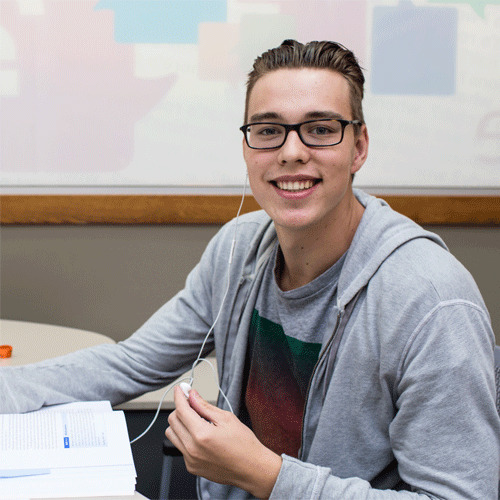
\includegraphics[width=0.4\textwidth]{kevin2.jpg}
\end{wrapfigure}
\textbf{\large Kevin Donnavan (23)} \\ \\
\textbf{Job Title: }Engineering Student\\
\textbf{Education:} 3rd Year Mechanical Engineering\\
\textbf{Experience:}
\begin{compactitem}
\item 3rd Year Mechanical Engineering
\item Summer internship as a junior structural engineer
\item Army reserves - Infantry
\end{compactitem}
\textbf{Skills:}
\begin{compactitem}
\item Problem Solving, Mathematics
\item Programming in Java, C\#, and C++
\end{compactitem}
\textbf{Goals:}
\begin{compactitem}
\item Obtain a good GPA and find a job in his field.
\end{compactitem}
\bigskip 
\textbf{Goals and Tasks user accomplishes}\\
Kevin says he just wants to get through his classes and get a decent GPA. Like everyone, his hardest classes mostly have to do with math (although he feels he is better than average). Kevin will be happy with anything that can make his math calculations easier.\\ \\
\textbf{Problem calculator solves} \\
The calculator helps Kevin get fast answers to difficult math problems he sees in class. Without a calculator, he is not sure how he would calculate the various functions that he sees on a daily basis. The calculator has to be precise enough so he can get the right answer to complex solutions of differential equations but he is not willing to wait - calculation must be near-instantaneous.
\pagebreak


\begin{wrapfigure}{R}{0.4\textwidth}
\includegraphics[width=0.4\textwidth]{tarek2.jpg}
\end{wrapfigure}
\textbf{\large Tarek Ghamzi (23)} \\ \\
\textbf{Job Title: }Engineering Student\\
\textbf{Job Title: }3rd year Electrical engineering student\\
\textbf{Education:} High School + CEGEP, currently in Electrical Engineering\\
\textbf{Experience:}
\begin{compactitem}
\item Subway
\item Pharmacist assistant
\end{compactitem}
\textbf{Skills:}
\begin{compactitem}
\item Problem Solving, Mathematics
\item Programming in C++ , and arduino 
\end{compactitem}
\textbf{Goals:}
\begin{compactitem}
\item Finish his degree with a good GPA
\item Find a job in his field
\end{compactitem}
\bigskip 
\textbf{Goals and Tasks user accomplishes}\\
Tarek claims that his main priority in life at the moment is to get his degree in Electrical Engineering. He claims that his field is heavily based on math, which he struggles with.
He aims to graduate with a higher than average GPA to gain an edge over others in his highly competitive field.\\ \\
\textbf{Problem calculator solves} \\
His calculator helps him in computing the high level mathematical functions that would take hours to solve by himself. It also helps him double check his answers for simple calculations.
Tarek claims that his calculator is with him at all times. Its accuracy, speed and comfort are of highest value to him.

\vspace{0.25in}

\pagebreak

\begin{wrapfigure}{R}{0.40\textwidth}

\includegraphics[width=0.40\textwidth]{arash.jpg}
\end{wrapfigure}
\textbf{\Large Arash Mohajer (28)} \\ \\
\textbf{Job Title: }2nd year Avionics Engineering student \\
\textbf{Education:} High School + CEGEP, currently in University\\
\textbf{Experience:}
\begin{compactitem}
\item Completed two internships at a company that manufactures Flight Simulators
\item Worked part time as a waiter
\end{compactitem}
\textbf{Skills:}
\begin{compactitem}
\item Mathematics, Physics
\item Technical Writing
\item Some experience programming in C\# and Java
\end{compactitem}
\textbf{Goals:}
\begin{compactitem}
\item Find more internships during his degree
\item Finish his degree in a reasonable amount of time
\item Save money for his future (manage personal finance)
\end{compactitem}
\bigskip
\textbf{Goals and Tasks user accomplishes}\\
Arash wants to finish his degree in Avionics as soon as possible so that he can get a good job in a field that he enjoys. He wants to continue taking part in engineering competitions and hackathons to learn more about his field and others and to meet other like-minded individuals. He wants to manage his personal finance in order to pay off the debt that he currently has from his university tuition. \\ \\
\textbf{Problem calculator solves}
While he is more focused on graduating than getting good grades in his classes, he has many math and physics intensive classes where he relies on a calculator. He uses a calculator at school for homework, projects and exams. He also uses a calculator for conversion between different units for engineering and physics problems. At home, he uses his calculator to manage his personal finances and to plan his future spending. 
\pagebreak

\begin{wrapfigure}{R}{0.40\textwidth}
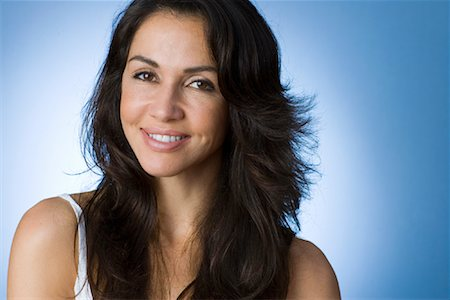
\includegraphics[width=0.40\textwidth]{victoria.jpg}
\end{wrapfigure}
\textbf{\Large Victoria Benlolo (35)} \\ \\
\textbf{Job Title: }1st year HR student\\
\textbf{Education:} High School + CEGEP\\
\textbf{Experience:}
\begin{compactitem}
\item Has owned and managed a spa for 2 years
\item Worked as a financial analyst for 7 years
\end{compactitem}
\textbf{Skills:}
\begin{compactitem}
\itemsep0em 
\item Economics, Business, Finance
\item Public Speaking
\item Investing
\end{compactitem}
\textbf{Goals:}
\begin{compactitem}
\itemsep0em 
\item Maximize the profit of her business
\item Invest in new profitable endeavours 
\item She is interested in opening new spas around town once her business grows more
\item Hire new employees and continue to manage the finances of her business
\end{compactitem}
\bigskip 
\textbf{Goals and Tasks user accomplishes}\\
Victoria wants to continue to grow her business and potentially start franchising her spa to open up new locations around the city. She wants to hire new talent in order to expand her finance team. Her day-to-day includes managing employees' pay, keeping inventory of products, paying bills and managing business income. Additionally, she wants to continue investing in the stock market. \\ \\
\textbf{Problem calculator solves}
At the Spa, Victoria uses a calculator to calculate all of her business expenses, profit/loss, employee salaries, etc. A reliable calculator is very important to her. She uses a calculator to plan expenses in her future business expansion plans.  She also uses a calculator to keep track of how her personal accounts and investment portfolios are growing. 
\pagebreak

\section{Use Cases}

With the initial requirements gathering step mostly completed, we were now able to arrive at a set of simple use cases. These would form the base of the functionality that we wanted to offer to the user.

\begin{center}
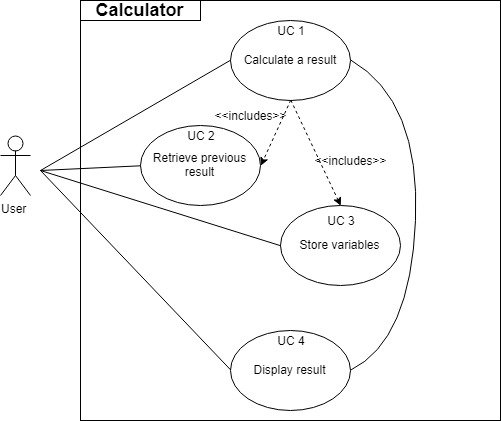
\includegraphics[width=0.5\textwidth]{UseCaseDiagram.jpg}
\end{center}

\begin{center}
Note: see appendix for full use case descriptions
\end{center}

\section{Design}

\subsection{Influence of Use Cases on Design Decisions}

The 4 use cases derived from the requirements gathering process undertaken in iteration 1 were the foundation of all design decisions. We knew that any design aspects that did not directly contribute to providing these use cases would be an extra feature at best or superfluous at worst.
\\

From UC1 (Calculate a result), we knew that there would be a module responsible for the math side of our calculator. UC 4 (Display result) naturally lead to the need for a GUI that could display the results and any errors that occurred during operation of the calculator. To meet UC3 (Store variables) would need a place to store these variables and the ability for the user to assign them. To us, UC2 (Retrieve previous result) seemed very simple and is the only one of the use cases that we did not anticipate needing its own structure.


\subsection{Macro Architecture}

At first, our calculator was going to be quite simple: a GUI with buttons that would call certain function and return the result. This original set of functionality was so simple that we could not see the need of a design pattern. It was after a careful review of the Personas that we saw the necessity of providing the users with the ability to type in their expressions directly into the GUI. This logically meant that we needed some sort of Parser to process these expressions and resolve each to a single number. This meant that we would need a significant module in between the GUI and the store of math functions. This module would effectively translate human-readable expression into a list of instructions for the machine to execute in the right order. We all knew which design pattern fit the job.
\\

MVC was chosen without any debate amongst us due to its perfect fit with our problem. We had a GUI interface that the user used to interact with the program (View). We had the store of math functions and constants that would be called as needed (Model). Lastly, translating human-readable expressions into instructions for the math functions (Controller).
\\

The main advantage we saw with MVC (apart from already fitting perfectly with what we wanted to make) was that it allowed us to decouple the coding effort. In reality, it allowed us to have one coder specialize on the GUI and another on the Parser. The was definite separation of concerns as our “GUI guy” did not need to know about what our “Parser guy” was up to. The two only ever needed to talk about the interface between the two modules. This was a significant time saver.
\\

Having everything separated also helped us to better organize our code. Things were easier to find and modify since we knew, for example, that all of the GUI and user-level functionality could be found in one place.


\subsection{Micro Architecture}


Note to reader: Please see annexes for detailed CRC class model of our code.
\\

With the macro architecture settled on the MVC pattern, we then needed to put together a micro architecture. To be quite honest, we did not put a great deal of thought into the design of the micro-level. We chock this up to our lack of experience and the fact that most of our calculator was coded before we covered that subject in class. If we had to start over, we would have put more time into the design before getting to coding. We hit a few unexpected hurdles that were directly due to our not explicitly setting out a class structure for our code. In our defense, there was a great deal we did not yet understand about the problem during what should have been a design phase. We learned while doing and in hindsight, a formal design based our very incomplete understanding of the solution space would have definitely been wrong.
\\

Regardless of our difficulties in the micro design, we were surprised to find that the CRC model was quite coherent and had very low coupling between the classes / modules. This is probably because we did our best to follow the macro architecture and have as few interfaces between the main modules of MVC. From this we concluded that a macro architecture, when followed closely, contributes to good order and discipline in the micro architecture.


\subsection{GUI Design and User Experience}

At the outset of our project, our team was faced with many questions regarding the user interface of our version of the Eternity calculator such as: Would our user interface be graphical or textual? Should the user interface emulate the look of a ‘real-life’ calculator? How would the calculator’s keys be mapped? Should the user interface be customizable? While designing and implementing our user interface we were tasked to answer these questions (and more) while adhering to principles of interaction design to ensure that our users have good experiences using our software. 
\\

\textbf{Textual or graphical?}

Once most of the mathematical functions were properly implemented before Deliverable 2, we wrote a simple textual user interface (TUI) that ran in the command line in order to test and demo our milestone build. We discussed as a team whether or not we would implement a GUI to replace our simple command line application. A TUI would be more lightweight, easier to implement and would only require a keyboard in order to function. It would also allow our users to see a history of their commands. However, a GUI is easier to use and more intuitive to a user, it is much nicer to look at and it would allow us to customize the interface more than a TUI. 
\\

After some discussion, we decided to implement a GUI using JavaFX because we wanted to be able to have full control over the look and feel of our calculator to give our users the best experience possible. We did want to integrate some functionality that we liked from the TUI like having the option to use a keyboard only and keeping a history of past expressions and answers.
\\

\textbf{Listening to our Users}

In order for our intended users to have good experiences with our application, we needed to listen to them and implement features that we know that they wanted in their ideal calculator. 
During the user interviews during Deliverable 1, we compiled several points that our interviewees made that we picked to become features in our user interface. 
\\

Firstly, two interviewees suggested that we add visual themes so that users could choose what version of the calculator they wanted to see. We designed one dark theme and one lighter theme since some users might have a preference between different contrasts. 

\vspace{5mm}

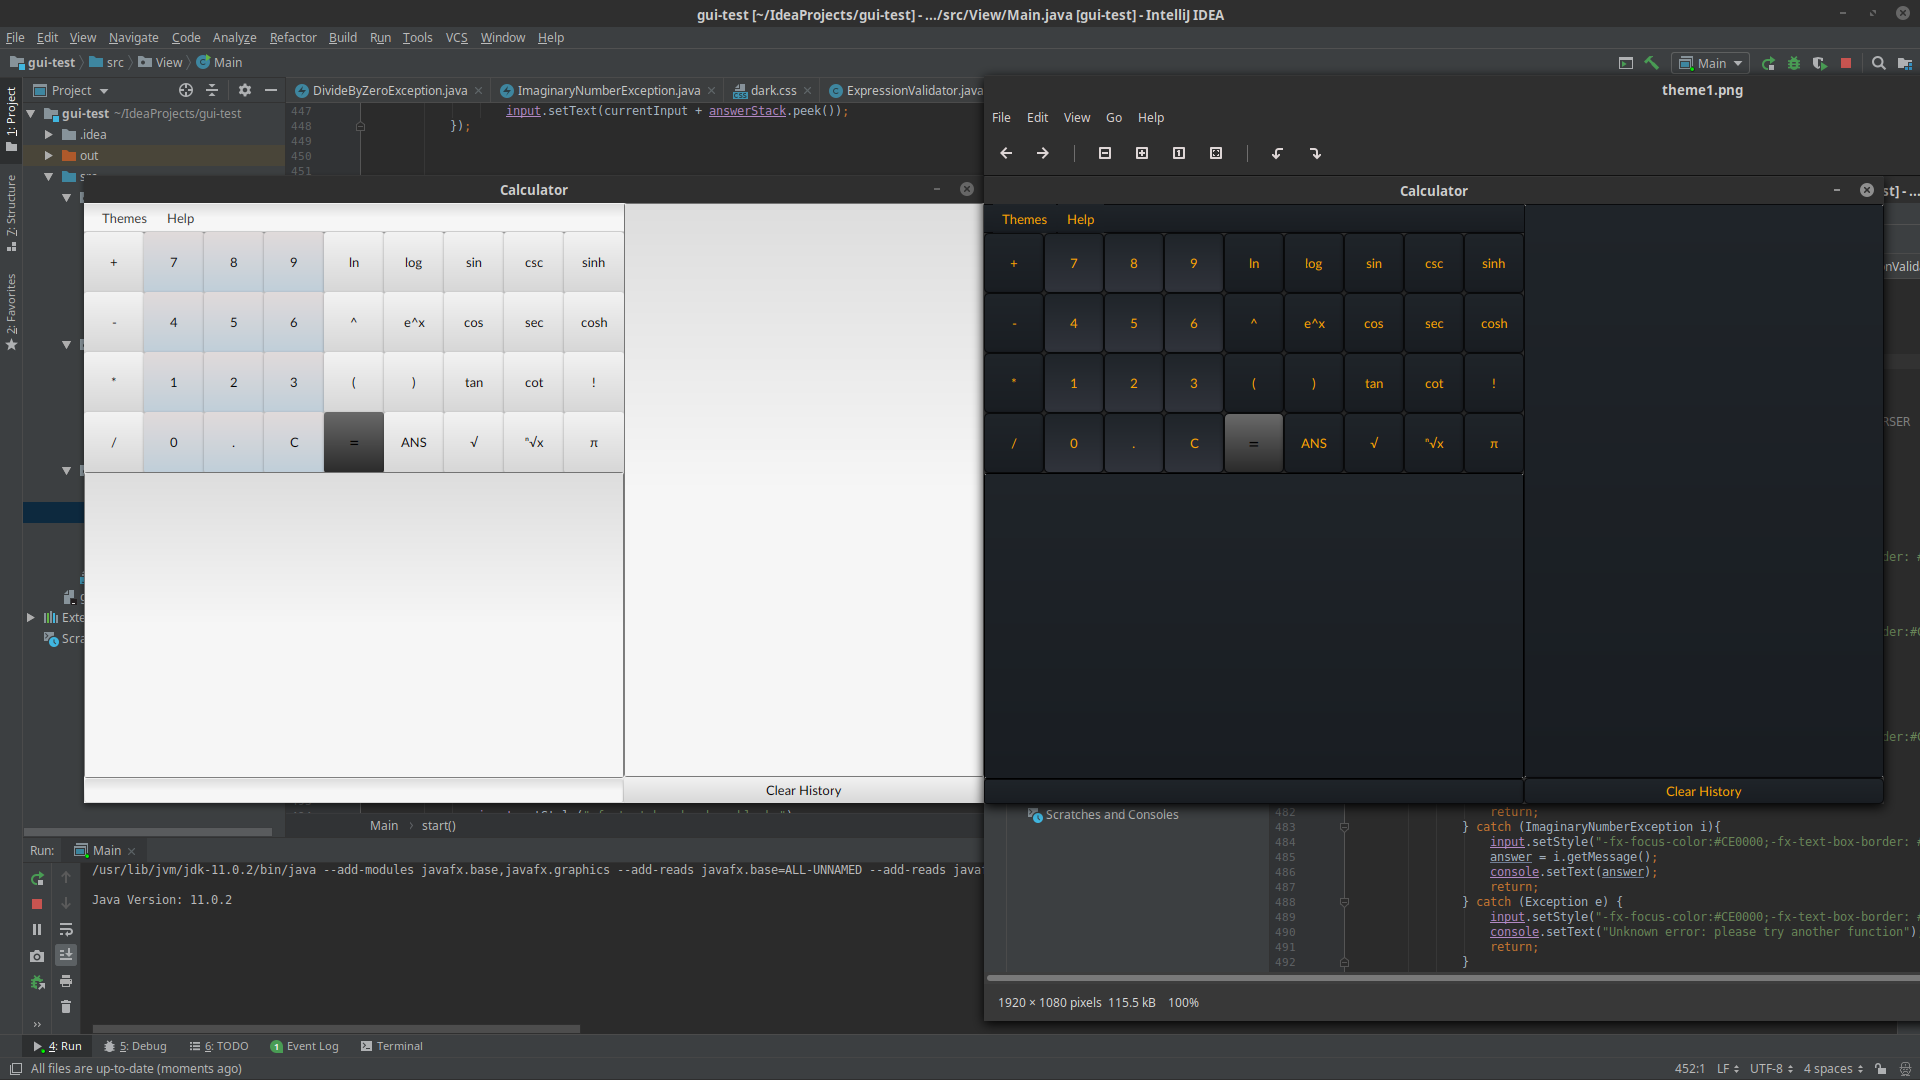
\includegraphics[width=0.80\textwidth]{themes.png}

\vspace{5mm}

Secondly, some of our interviewees wanted to be able to type in their mathematical functions with their keyboards. This encouraged our decision to make an expression parser and input field for our users to be able to use all functions of the calculator without using their mouse. 
\\

Finally, we had several people tell us that they were familiar with the look of regular pocket calculators so we based our calculator button layout on existing calculators that we had used in the past.





\section{Implementation}

\subsection{Roadblocks During Implementation}

During the implementation of the planned architecture, several roadblocks appeared some of which could be ignored, some which could be dealt with, and some that forced a change in the architecture itself.
\\

The first roadblock we encountered was during the design stage of the power function.The problem was that when the power function received an exponent with many decimal values, the software would stall. After an extensive use of the debugger, we were able to trace back the problem to our  intPower function, which calculates the power, but only accepts exponents of integer type. Thus we used the IntPower function within the primary power function to help calculate expressions correctly. The problem arises when the power function is given an exponent with lots of decimal values, due to the way it functions, it ends up passing an extremely large exponent to the intPower function, which ends up stalling it. Therefore the intPower function’s performance had to be improved. Upon research we discovered an algorithm called “exponent by squaring ”  that is much more efficient than the one used in the intPower, which we ended up using to solve our problem.
\\

Another issue that was found in the power function was that when given a large exponent, the answer ends up being slightly inaccurate. The problem was both a mathematical and hardware one. As we know computers are not perfectly accurate when calculating numbers, but usually the offset is too small to matter. However in a power function, that offset grows exponentially, which ends up with the final answer having a significant offset. It was decided to leave such a problem unattended since it was too costly in terms of time and resources to fix, but mainly because the offset, compared to the final answer, was too small to make a difference.
\\

During our time working on the project, we encountered another roadblock that had to do with the nroot function, responsible for calculating the nth root of a number. The problem was that some functions,in certain cases, relied on it to calculate, for instance, the 10,000th root of a number, which obviously stalled the software. The solution we found only worked when the exponent was a multiple of 10, however it was good enough since the functions that rely on the nroot function complied with such restrictions. The solution consisted of creating a seperate function that instead of calculating the 10,000th root right away, it splits it by calculating the 10th root iteratively, a calculated amount of times, and ends up giving the right answer in a relatively short amount of time. 
\\

After the basic math functions were implemented, and work was started on the parser, we realised that if a user gave an improperly formatted input, there was a potential to crash the software. For this reason it was decided that our program had to have a way to verify the user input as well display the appropriate error messages, hence an expression verifier had to be added to our initial designs, and implemented later on.
\\

The coders responsible for the ExpressionValidator and the Parser respectively spend a great deal of time manually parsing Strings. In fact, around 30\% of the effort of those respective classes was spent on String manipulation of all sorts. The team only learned of the Java Regex API (Pattern and Matcher classes) at the very end of the project. The use of these tools would have greatly enhanced our productivity and probably allowed us the leeway to include some added features.

\subsection{Adjustment to the Micro Architecture}

As was mentioned in the section detailing the micro architecture, we did not have a full picture of the microstructure of our calculator before we started coding it. This meant that we did not have a fully fleshed out design to go by and had to develop one iteratively. 
\\

One crucial element we had not foreseen was that the String expression entered into the calculator by the user would not be “clean”. This meant that we would need to validate it for syntactical correctness and do some light formating to simplify the Parser’s job. Our initial estimates for this validation step were 2-3 days of effort at most. As things are wont to do, this turned into 2-3 weeks. We assigned one coder to the validator functions and in the first night, he had come up with 10 scenarios that we had not anticipated. We figured that there were probably a few more scenarios hiding out so we convened a meeting to brainstorm every possible case that a user could mess up in his/her input. This coder ended up spending a good part of the project on this one method (a method that would call 17+ other methods). This was a significant time sink that had not been planned. Furthermore, as we tested, we kept coming up with new ways to break the Parser with user input. The validator function grew in tandem. This was by far the largest unanticipated addition to our micro architecture.
\\

Another micro architectural decision we made during this iteration was to consolidate all math functions into a single class. We did this after it became a giant paint to track down which function was in which class (MathFunctions or TranscendentalFunction). We gave it a good think as a group and unanimously concluded that there was no good reason not to put them all in the same place.
\\

We also reduced the quantity of Exception classes we used. Rather than have multiple classes, we settled on MathExceptions and SyntaxExceptions which would have individual instances of helpful messages (ie. if dividing by 0 throw new MathException(“Error: Division by zero”);. This made a code much more manageable and would make the CRC diagram smaller.


\subsection{Outstanding Issues}

Over the course of our project we faced some challenges that we were unable to fix. Some were due to aiming for goals that proved to be too ambitious and some due to programing language limitations, however most of them were due to time limitations constraints.
\\

One of such issues was our comma validation in the expression validator. Our plan was to have the root and log functions accept 1 value , in which case the square root and log(base 10) functions would be called respectively, or the user would have the option to give the functions 2 parameters, separated by a comma, to have the option of calculating the nth root of a number or a log of base other than 10. For that reason it was decided that our parser should have the functionality to handle commas in strings , and the expression validator to validate commas. Fortunately we were able to integrate such functionality into the parser, and the calculator functions properly as long as the user uses commas in the proper format, however , due to time constraints, we were not able to include such functionality in the expression validator. Therefore if the user utilises commas in the improper format, the behaviour of the calculator is unpredictable.
\\

Another minor issue we discovered was that our GUI framework (JavaFx) was not supported past Java 8. (the technical reason we were told was that the JVM was slightly altered in a way that made running JavaFx code difficult or impossible). This was not a major issue for most of the coders but our “GUI guy” was on version 9 and it took him a few days to find out why he could not build our project into a JAR. Reverting to Java 8 fixed the issue but it imposes a limitation on users running our JAR: they must be using Java 8 or less.


\section{Testing}

\subsection{Usefulness of Debugger in Testing}

Every coder reported the usefulness the debugger functions in their respective IDEs (see appendix for screenshots). This was because this was a larger and more complex project than any of us had done before. Compounding this was the total separation of tasks among the coders meaning that a coder may be responsible for functionality downstream of his colleague’s codes. The downstream coder would not have a firm grasp on all possible input into his code then. This made the debugger essential to getting visibility on what was going on inside our code.
\\

The debugger was used most often to check the flow of the ExpressionValidator and the Parser since they were the more error-prone parts of the code. It was also greatly appreciated in most loops to check for edge cases causing out-of-bounds errors.
\\

Debugger were very useful in examining specific failure cases in our math function unit tests. Since we used some Taylor expansions, certain inputs gave us unexpectedly poor precision results. The debugger helped the team isolate these problems and put us on the path to improving our algorithms for these edge cases.

\subsection{Unit Testing}

Once we had implemented our transcendental math functions, we needed a way to reliably and quickly test a large range of inputs against them to validate that our results made sense.  
\\

In order to accomplish this, we wrote several unit tests for each function spanning ranges of inputs both inside and outside of each function’s mathematical domain. We also had to determine a universal acceptable accuracy was for our results across all of our functions. This was important for us so that we could have a consistent amount of significant figures between different calculations. After quickly testing several of our math functions, we decided that having seven figures after the decimal was a sufficient and realistic amount of accuracy that all the functions we wrote could accurately output.
\\

We used JUnit, a Java library that integrates into several IDEs to write these tests. The JUnit integration into IDEs provided us with a quick way to write, compile and get results efficiently.
\\

\textbf{Unit Testing Example:}
\\
For our logarithmic function (ln), since its domain is from 0 to positive infinity, we wrote unit tests calculating values from that range using our function and Java’s ln function (from java.lang.Math) to compare results and ensure that our function was accurate up to seven digits after the decimal. Additionally, we tested our functions with transcendental numbers such as Pi and Euler’s constant. We employed a similar unit testing strategy for all the math functions that were implemented.

\vspace{8mm}
\begin{centering}
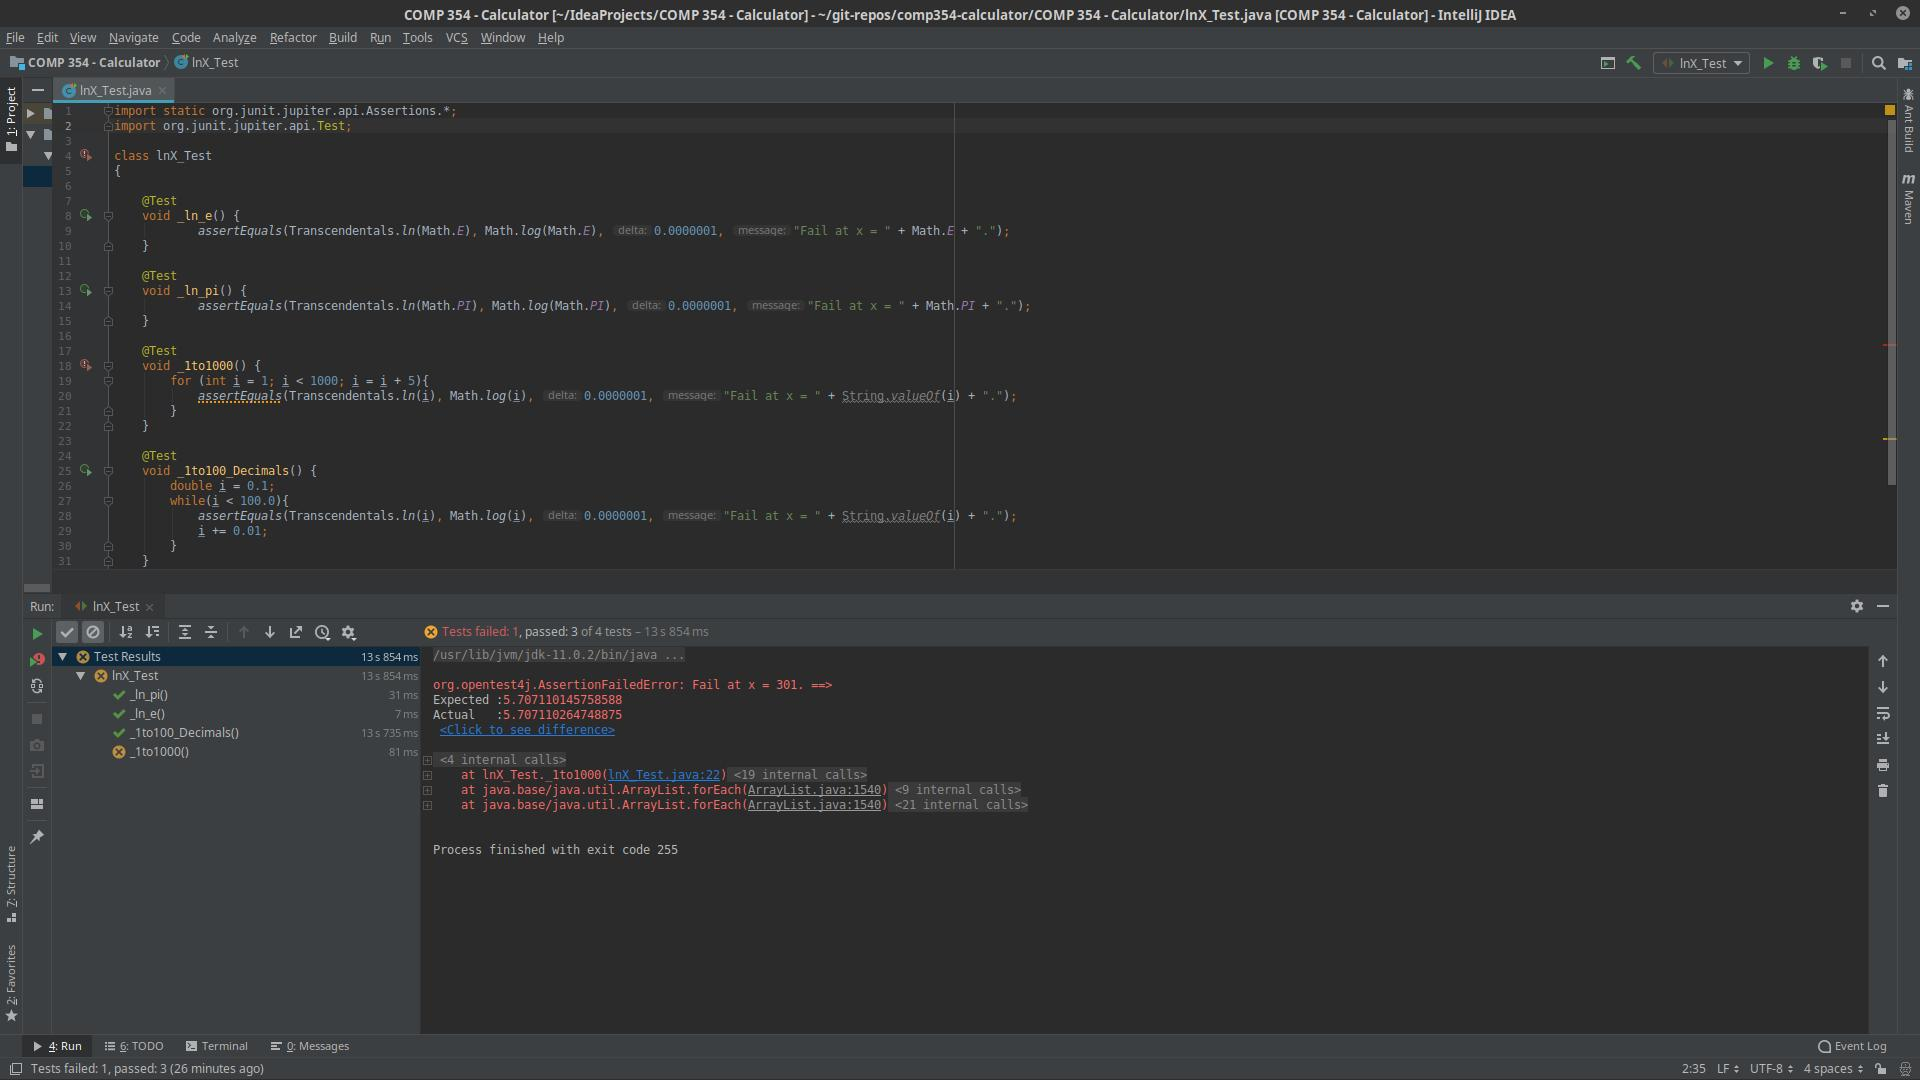
\includegraphics[width=0.9\textwidth]{Testing_1.jpg}
\end{centering}
\vspace{8mm}

Unit tests proved to be very useful in isolating individual functions outside of the overall application's context to validate that they were calculating not only correct but sufficiently accurate results. They also allowed us to diagnose issues or inaccuracies quickly in our code editor and make changes to our code. This was an extremely important step to making for an efficient iteration cycle.



\subsection{Integration Testing}

Once we had ironed out most of the issues within our individual functions, we integrated these with our user interface, expression validator and expression parser to validate that all parts were working together properly. Integration testing also allowed us to test certain scenarios in which we could not efficiently write unit tests for. Before testing, each team member explained the expected functionality of the module that they worked on and once we all had a basis for how the entire system should work, we went to work testing various scenarios that made use of every different part of the software system. 
\\

\textbf{Testing the Expression Validator}

The expression validator had a responsibility to make sure that the string being passed to it was a valid, syntactically correct mathematical expression so that it could be handed over to the expression parser. In order to test its functionality, we tested inputting strings such as:
\\

\begin{itemize}[noitemsep,topsep=0pt,parsep=0pt,partopsep=0pt]
\item Strings with mathematically irrelevant characters such as $\#$, $\&$, full words, etc.

\item Unmatched bracket combinations such as $()($, $)))$, etc.

\item Expressions that do not make sense such as $2++3$, $4-$.
\end{itemize}

\vspace{5mm}

These input strings should all throw exceptions, display an error message to the user and, most importantly, not pass the input string to the parser. If any of these did not catch an error and sent the erroneous string to the parser, we would debug and re-test until the issue was fixed.
\\

On top of testing incorrect strings, we also tested many different valid mathematical expressions to ensure that there would not be any exceptions thrown mistakenly. Additionally, this would allow us to test that the parser.
\\

\textbf{Testing the Expression Parser}

With the input strings being validated by the expression validator, we assumed that the input strings were syntactically correct mathematical expressions. This assumption allowed us to focus our testing on actual mathematical requirements, such as:
\\

\begin{itemize}[noitemsep,topsep=0pt,parsep=0pt,partopsep=0pt]
\item Combining different functions such as $sin(90)/ln(23)$, $sqrt(64)+Pi$, etc.
\item “Nesting” functions in other functions: $ln(cos(2))$, $e^(sinh)$
\item Respecting order of operations: $2*4+5$, $12 * ( 5 + 3 )$.
\item Mathematical errors such as dividing by zero, using inputs outside of certain functions’ domains, etc. 
\end{itemize}

\vspace{5mm}

We used online expression calculators to compare the results of these types of expressions to the real answers.  Furthermore, we needed to ensure that after calculating longer expressions with multiple functions, our results were still accurate to a reasonable degree and any math errors (such as dividing by zero) were handled by an error message. Testing our parser in this pseudo-random fashion allowed us to find several issues that were not caught in our unit tests.
\\

Integration testing was vital for zeroing in on issues that could have only been found with the entire system consolidated. Through this layer of testing, we found many edge-case issues from combining math functions and using different syntax, developed a more robust error messaging system and ensured that all parts of the system were working in harmony together.


\subsection{Acceptance Testing and Usability Evaluation}

In order to review how successful the implementation of our calculator has been, we needed to refer to at least 1 person in each category of the personas to provide us with feedback. This would allow us to find out if we were meeting their wants/needs and also to give us a better idea of what aspects we would have to work on in the future in order to continue improving our product.
\\

For our Technical/Mathematical user, Kevin Donnavan, he suggested that we make the keys mappable even though we were not able to implement it this time around. He believed it was an important feature that would make the calculator easier to use and customize for himself. What he liked was how the GUI was designed. He liked that the user input window was on the bottom opposed to the top, and he felt it encouraged him to want to use the keyboard more instead of using the mouse to click on the calculator buttons to calculate. He said it was a “solid stepping stone towards creating a customizable calculator where you have mappable keys for the user.” In other words, if we were to move forward with another iteration of our calculator, we’d want to focus a lot more on how the user would interact with it to strength customizability. 
\\

For our common/casual user, Victoria Benlolo, she suggested we make the application available for phones, not just computers, because one of her past suggestions, was to make the calculator as simple and portable as possible. She liked the idea that she could access it on her computer, but she wouldn’t be able to make calculations on the go if this was the only platform she could access it on. What she did like was the fact the we included all the functions she needed for her day to day business tasks, and complimented us on how clean the GUI looked. So overall, what we gathered from her 2nd interview was that we would have to put more emphasis on the portability of our product. 
\\

For our Academic user, Sarah Garrel, she was very impressed with the customizable skins provided for the calculator GUI. She mentioned she would like a wider range of coloured options, but overall she was impressed we implemented the feature she asked for in the first place. She suggested we still consider adding the key mapping feature to make it easy for her to customize the keyboard to a format that would compliment the courses she takes in University. In other words, she pointed us towards the direction of continuing to improve  on our calculator’s customizability and personification attributes. 


\section{Plans for Future Iterations}

To conclude, we learned a great amount throughout this project. From finding ways to strengthen our team dynamics to learning to appreciate the amount of thought and effort that goes into creating a calculator, we experienced it all. We are proud of the amount of work we were able to dedicate into this, but there is a lot we would’ve liked to have completed before the due date. For example, it would’ve been great to have had a chance to make our application available online to have had a better means of testing our features on multiple users, and not only our interviewees/personas.
\\

In addition, didn’t get to make our keys mappable even though it was a feature we knew was very desirable through our interviews. The reality though, was that this was a very ambitious feature to want to add in for a project we only had 12 weeks to implement. If our goals were more realistic and if we would’ve put a greater emphasis on feasibility, we would’ve predicted that it wouldn’t be possible to accomplish in such a short amount of time since most of our time was going to be spent on the fundamental aspects of creating a functional calculator. 
\\

Lastly, analyzing the feedback our persona interviewees provided us with, it’s clear that some of the nexts steps we can take to improve our calculator could be to focus on the UX (user experience) to create an engaging, portable, and personalized tactile experience! 
\\

With that said, in regards to the future plans for our Eternity Calculator, if we were to work on it in the future, we’d definitely want to improve its overall UX experience. Simply, after gathering all our data from our own experience and the feedback of others, this would be done by implementing key mapping, more customizable skins, making our calculator available online, and making it available for different platforms like smartphones. From there we’d be able to take it even further and continue building on this great experience we executed in 12 weeks.

\pagebreak

\section{Appendices}

\subsection{Appendix A - Use of a Debugger}

\begin{figure}[H]
\centering
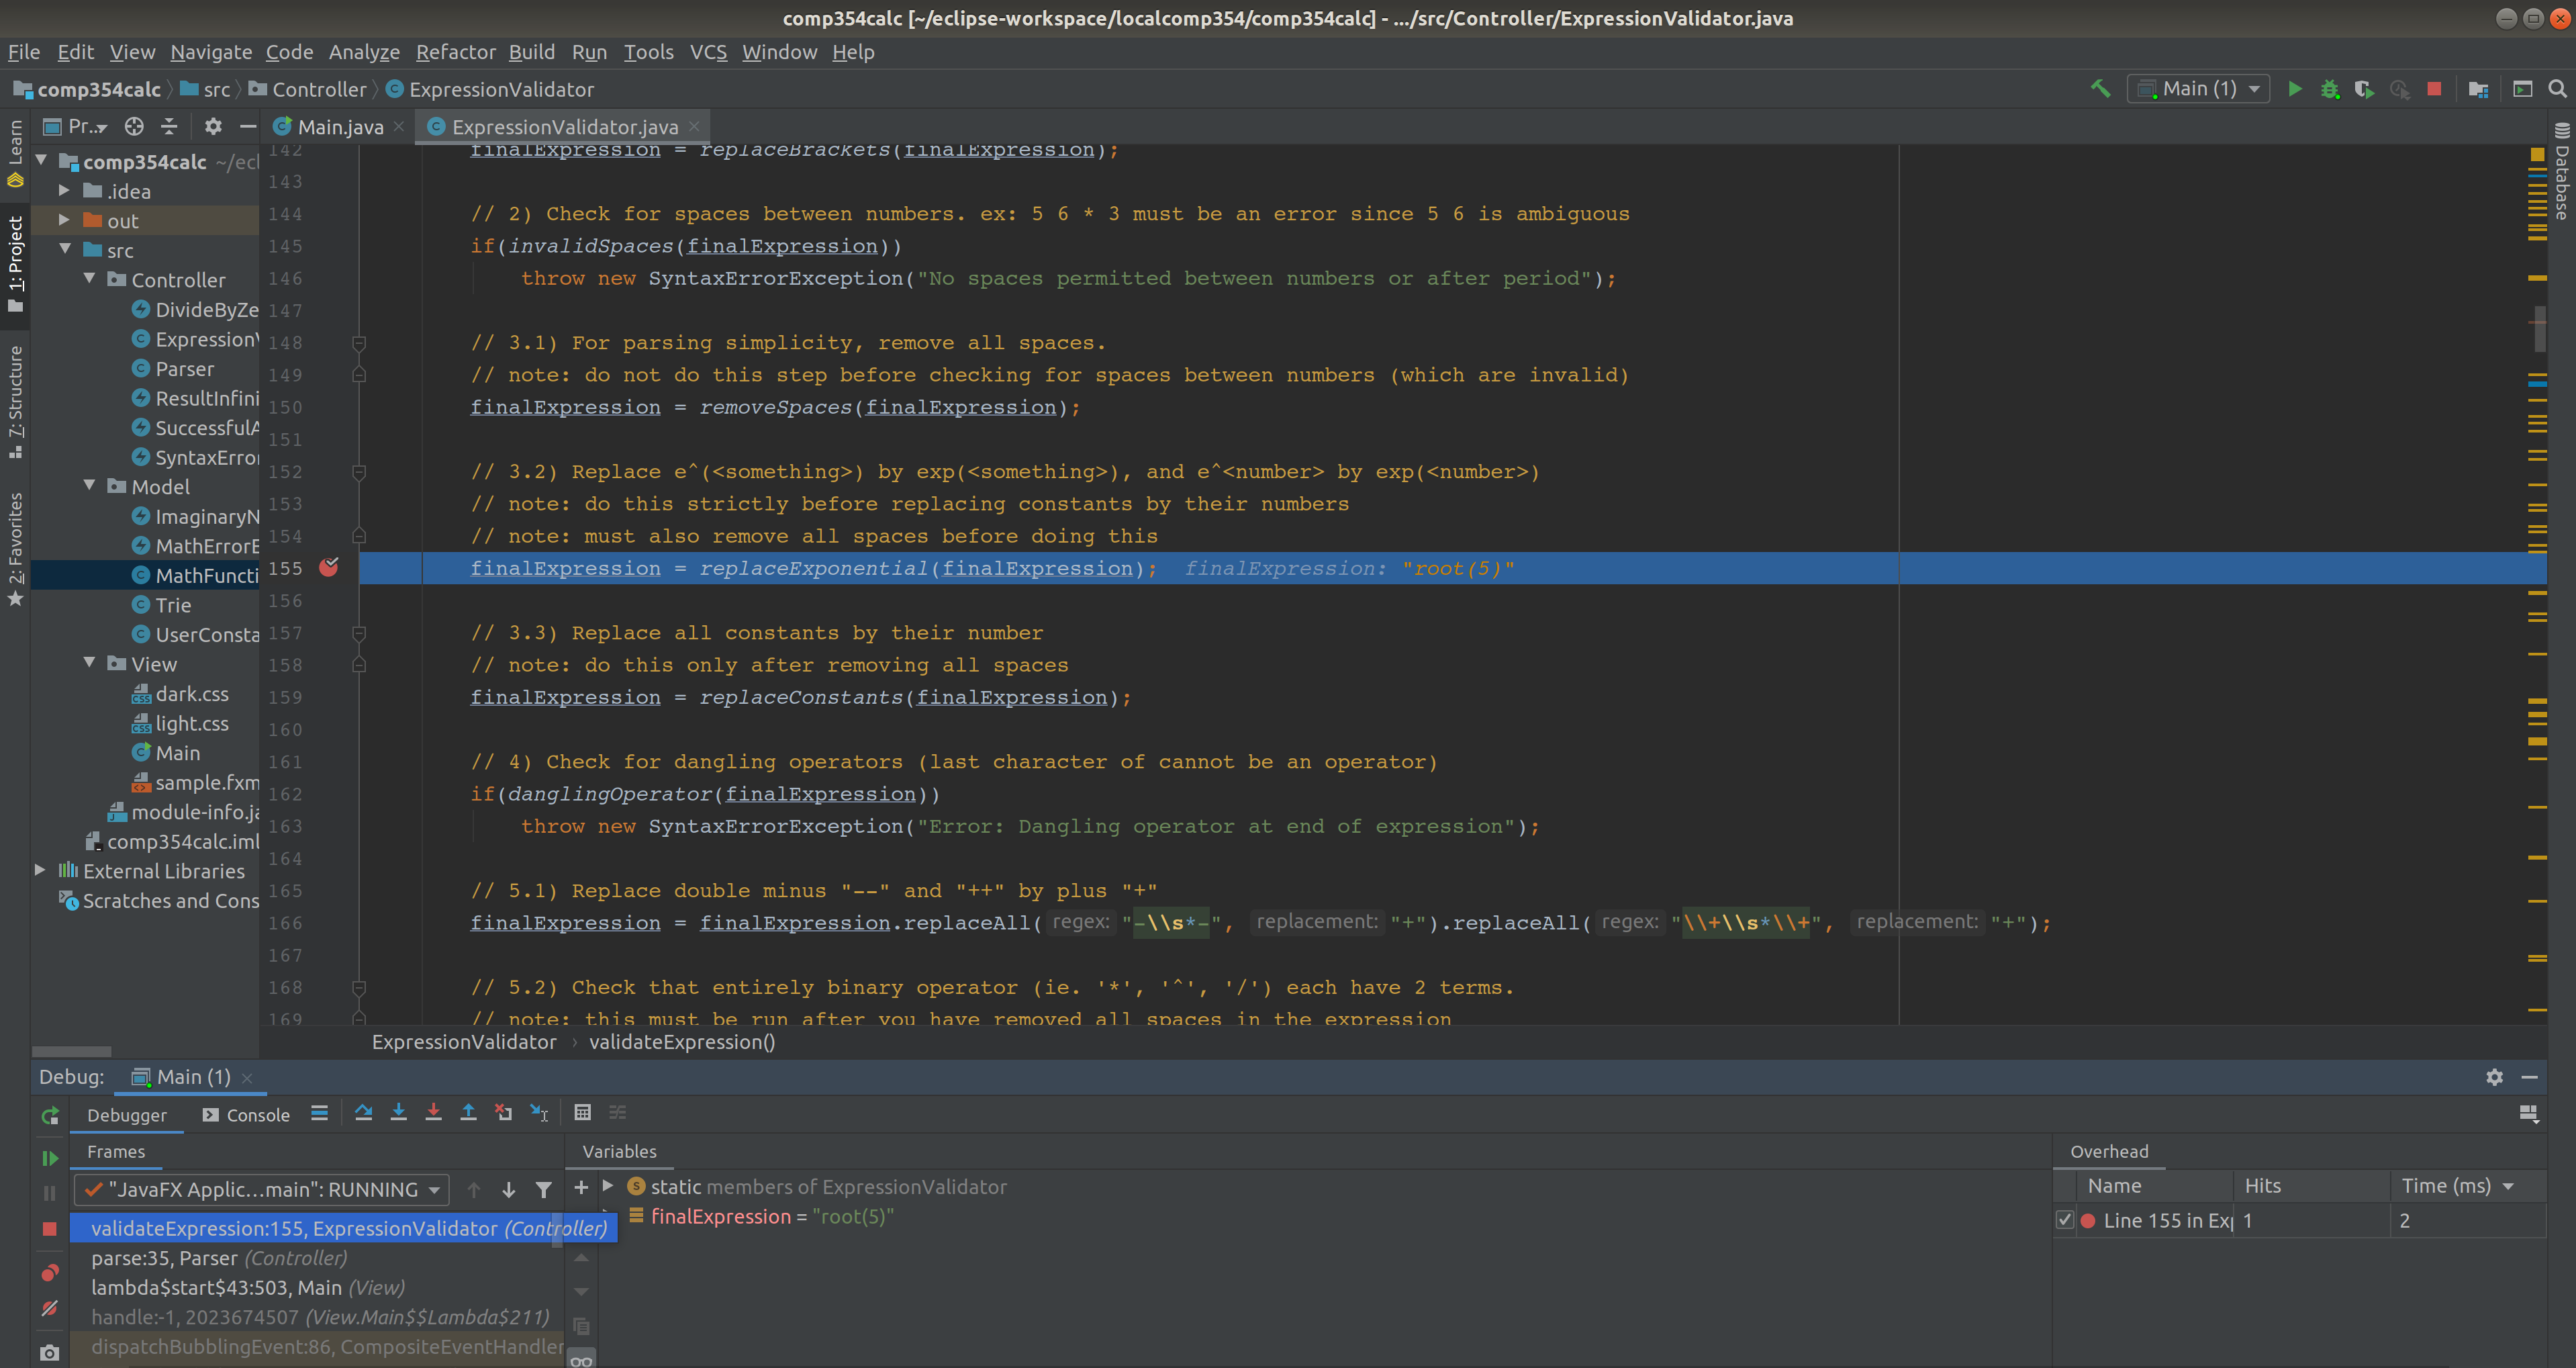
\includegraphics[width=1.13\textwidth]{dan1.png}
\caption{Daniel TS debugging why e\textasciicircum X is not being replaced by exp(X)}
\label{Dan1}
\end{figure}

\vspace{20mm}


\begin{figure}[H]
\centering
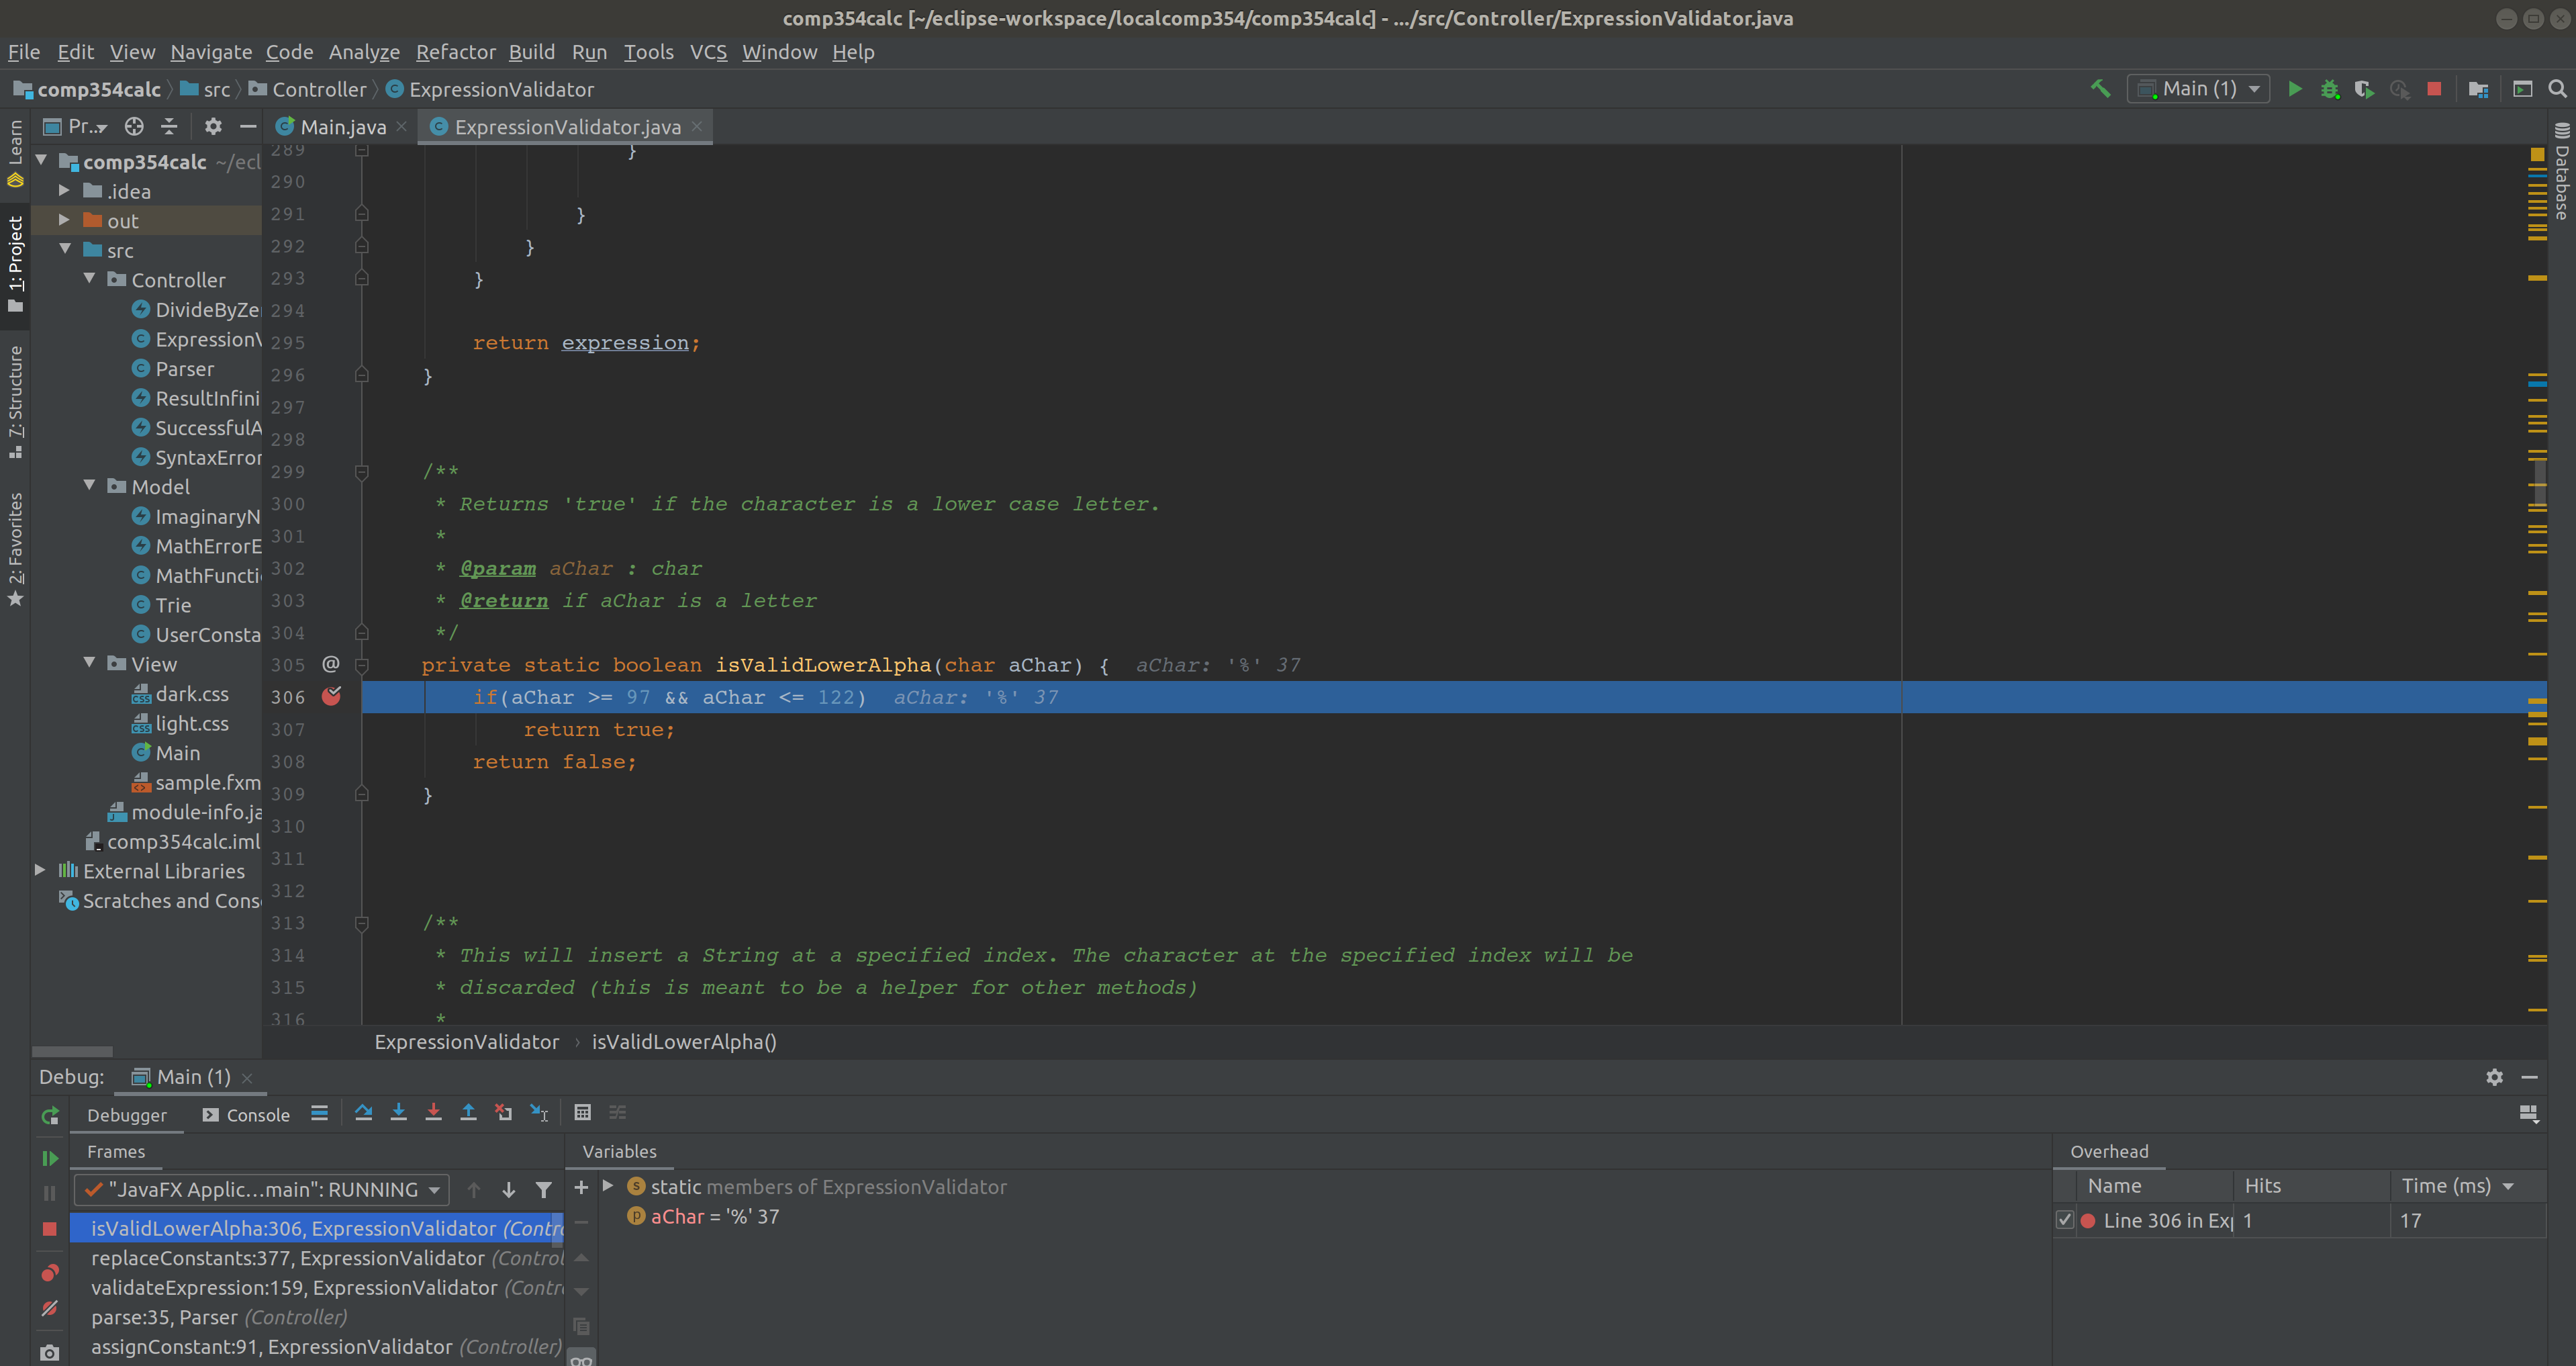
\includegraphics[width=1.13\textwidth]{dan2.png}
\caption{Daniel TS using debugger to check if his function checks for reserved characters}
\label{Dan2}
\end{figure}

\vspace{20mm}
\begin{figure}[H]
\centering
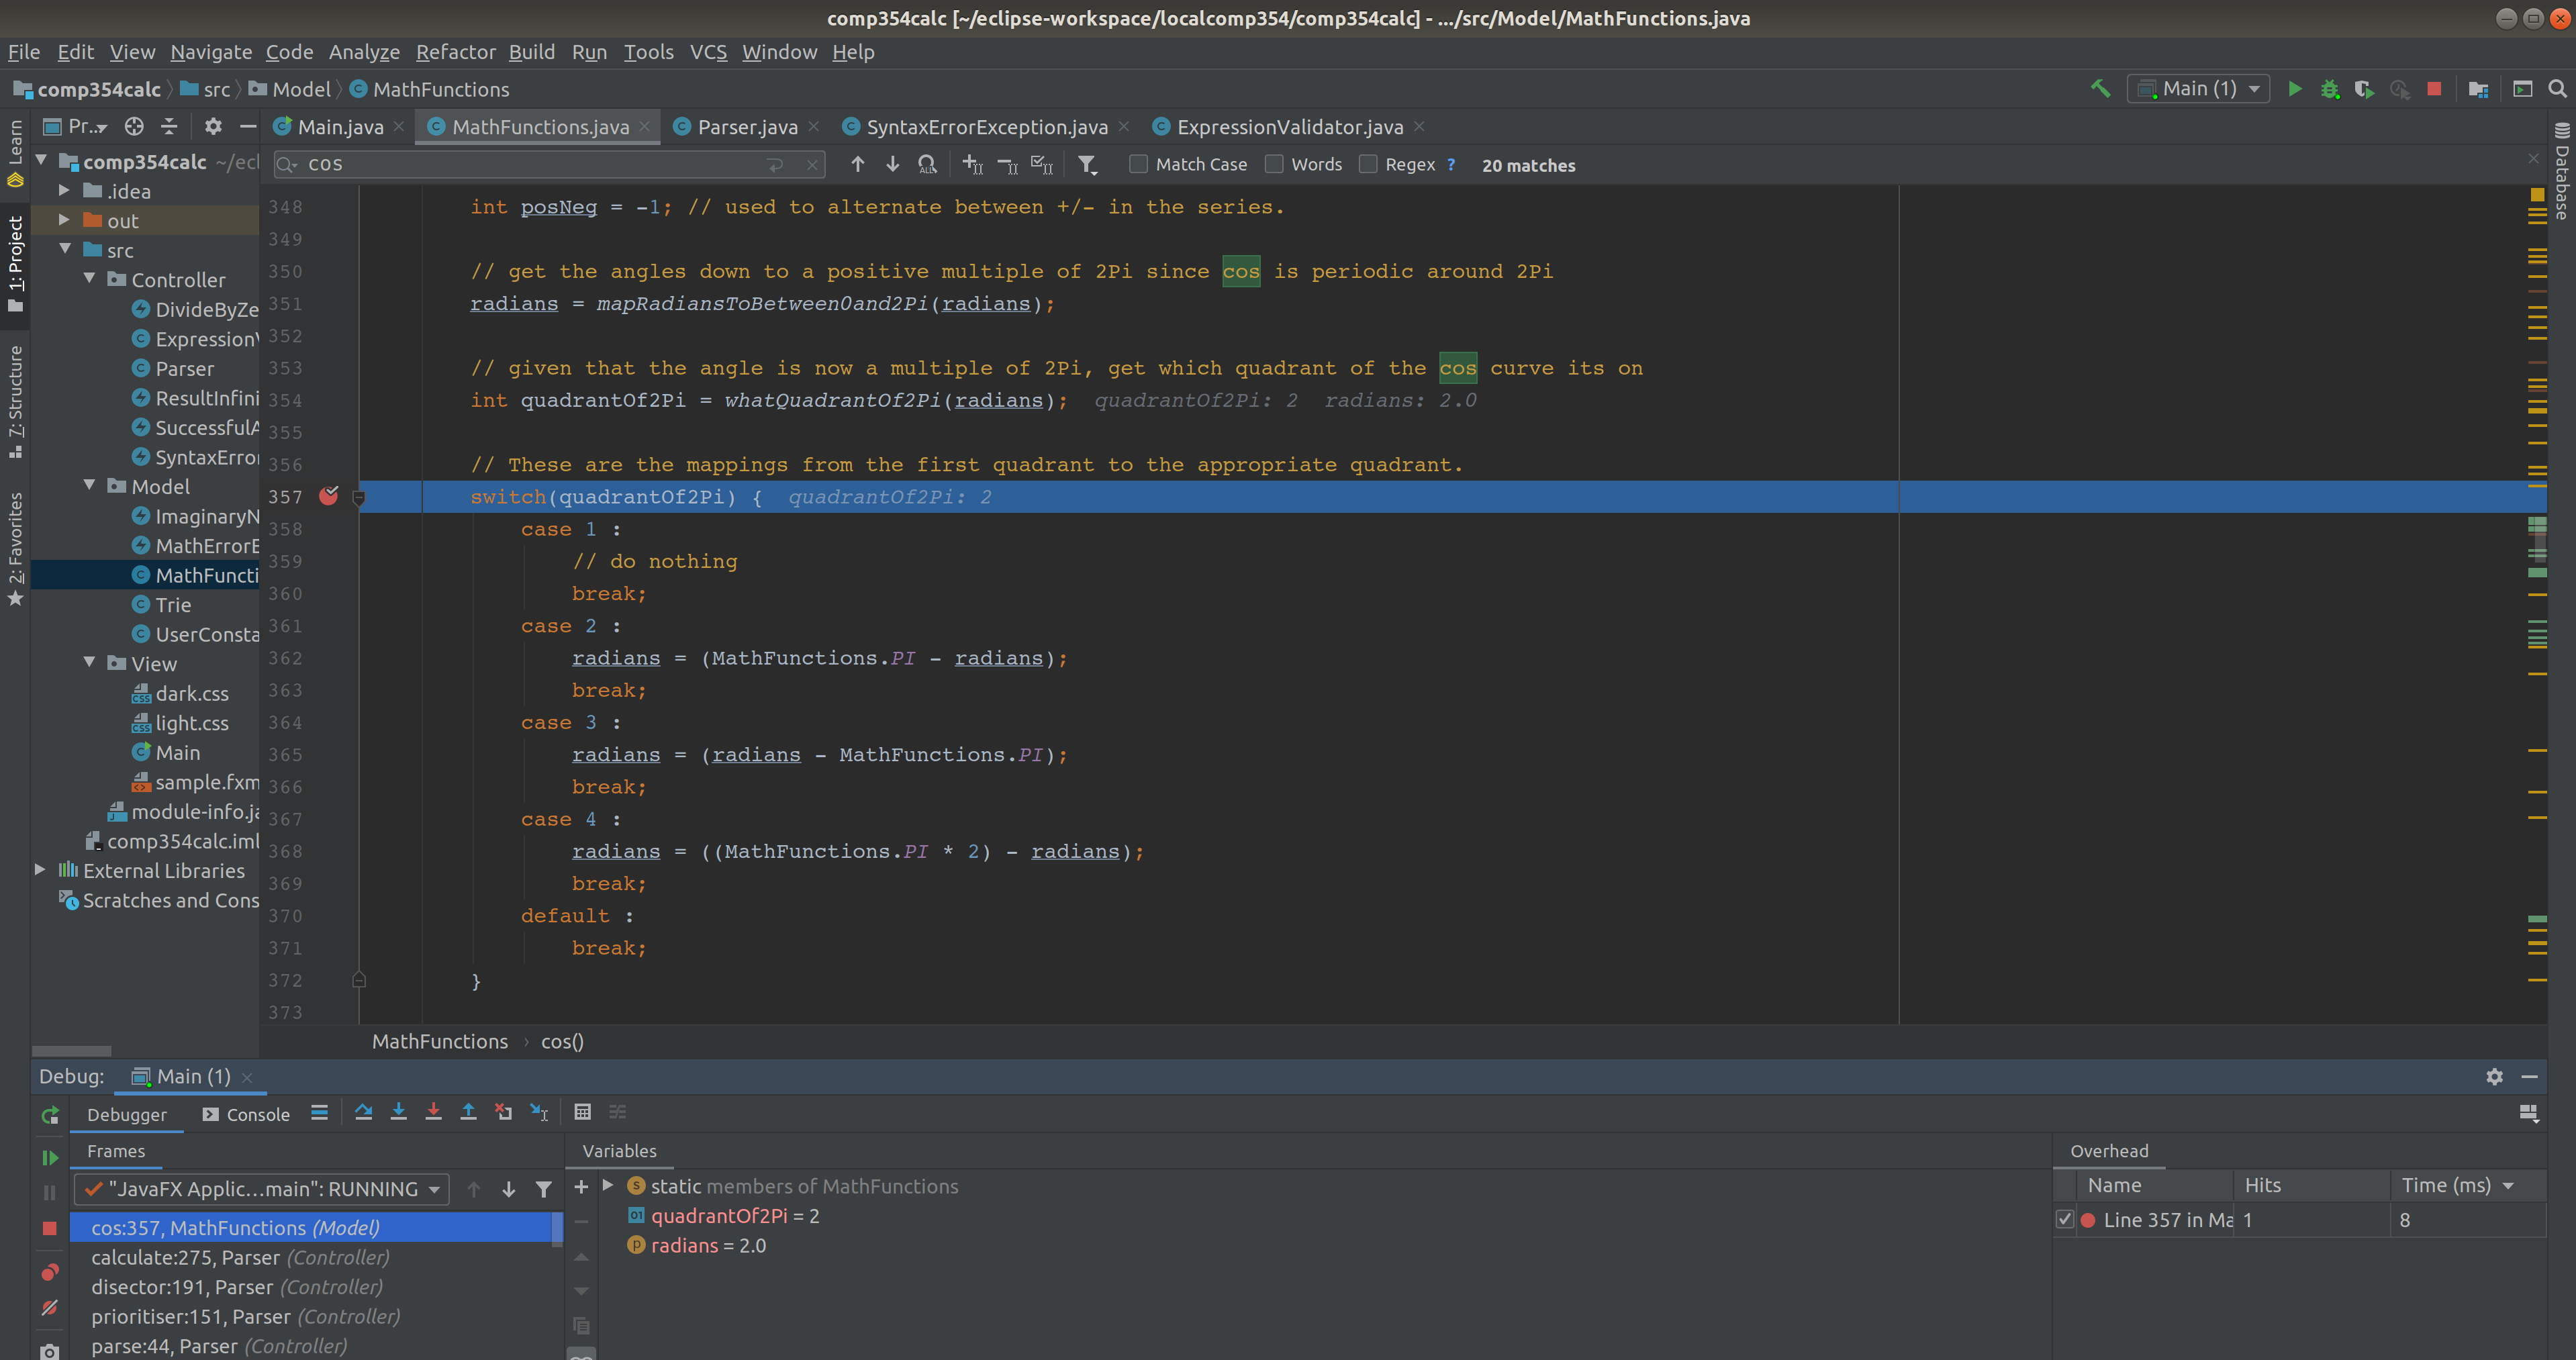
\includegraphics[width=1.13\textwidth]{Andres1.png}
\caption{Andres using the debugger to fing the bug in the cosine function}
\label{Andres1}
\end{figure}


\vspace{20mm}
\begin{figure}[H]
\centering
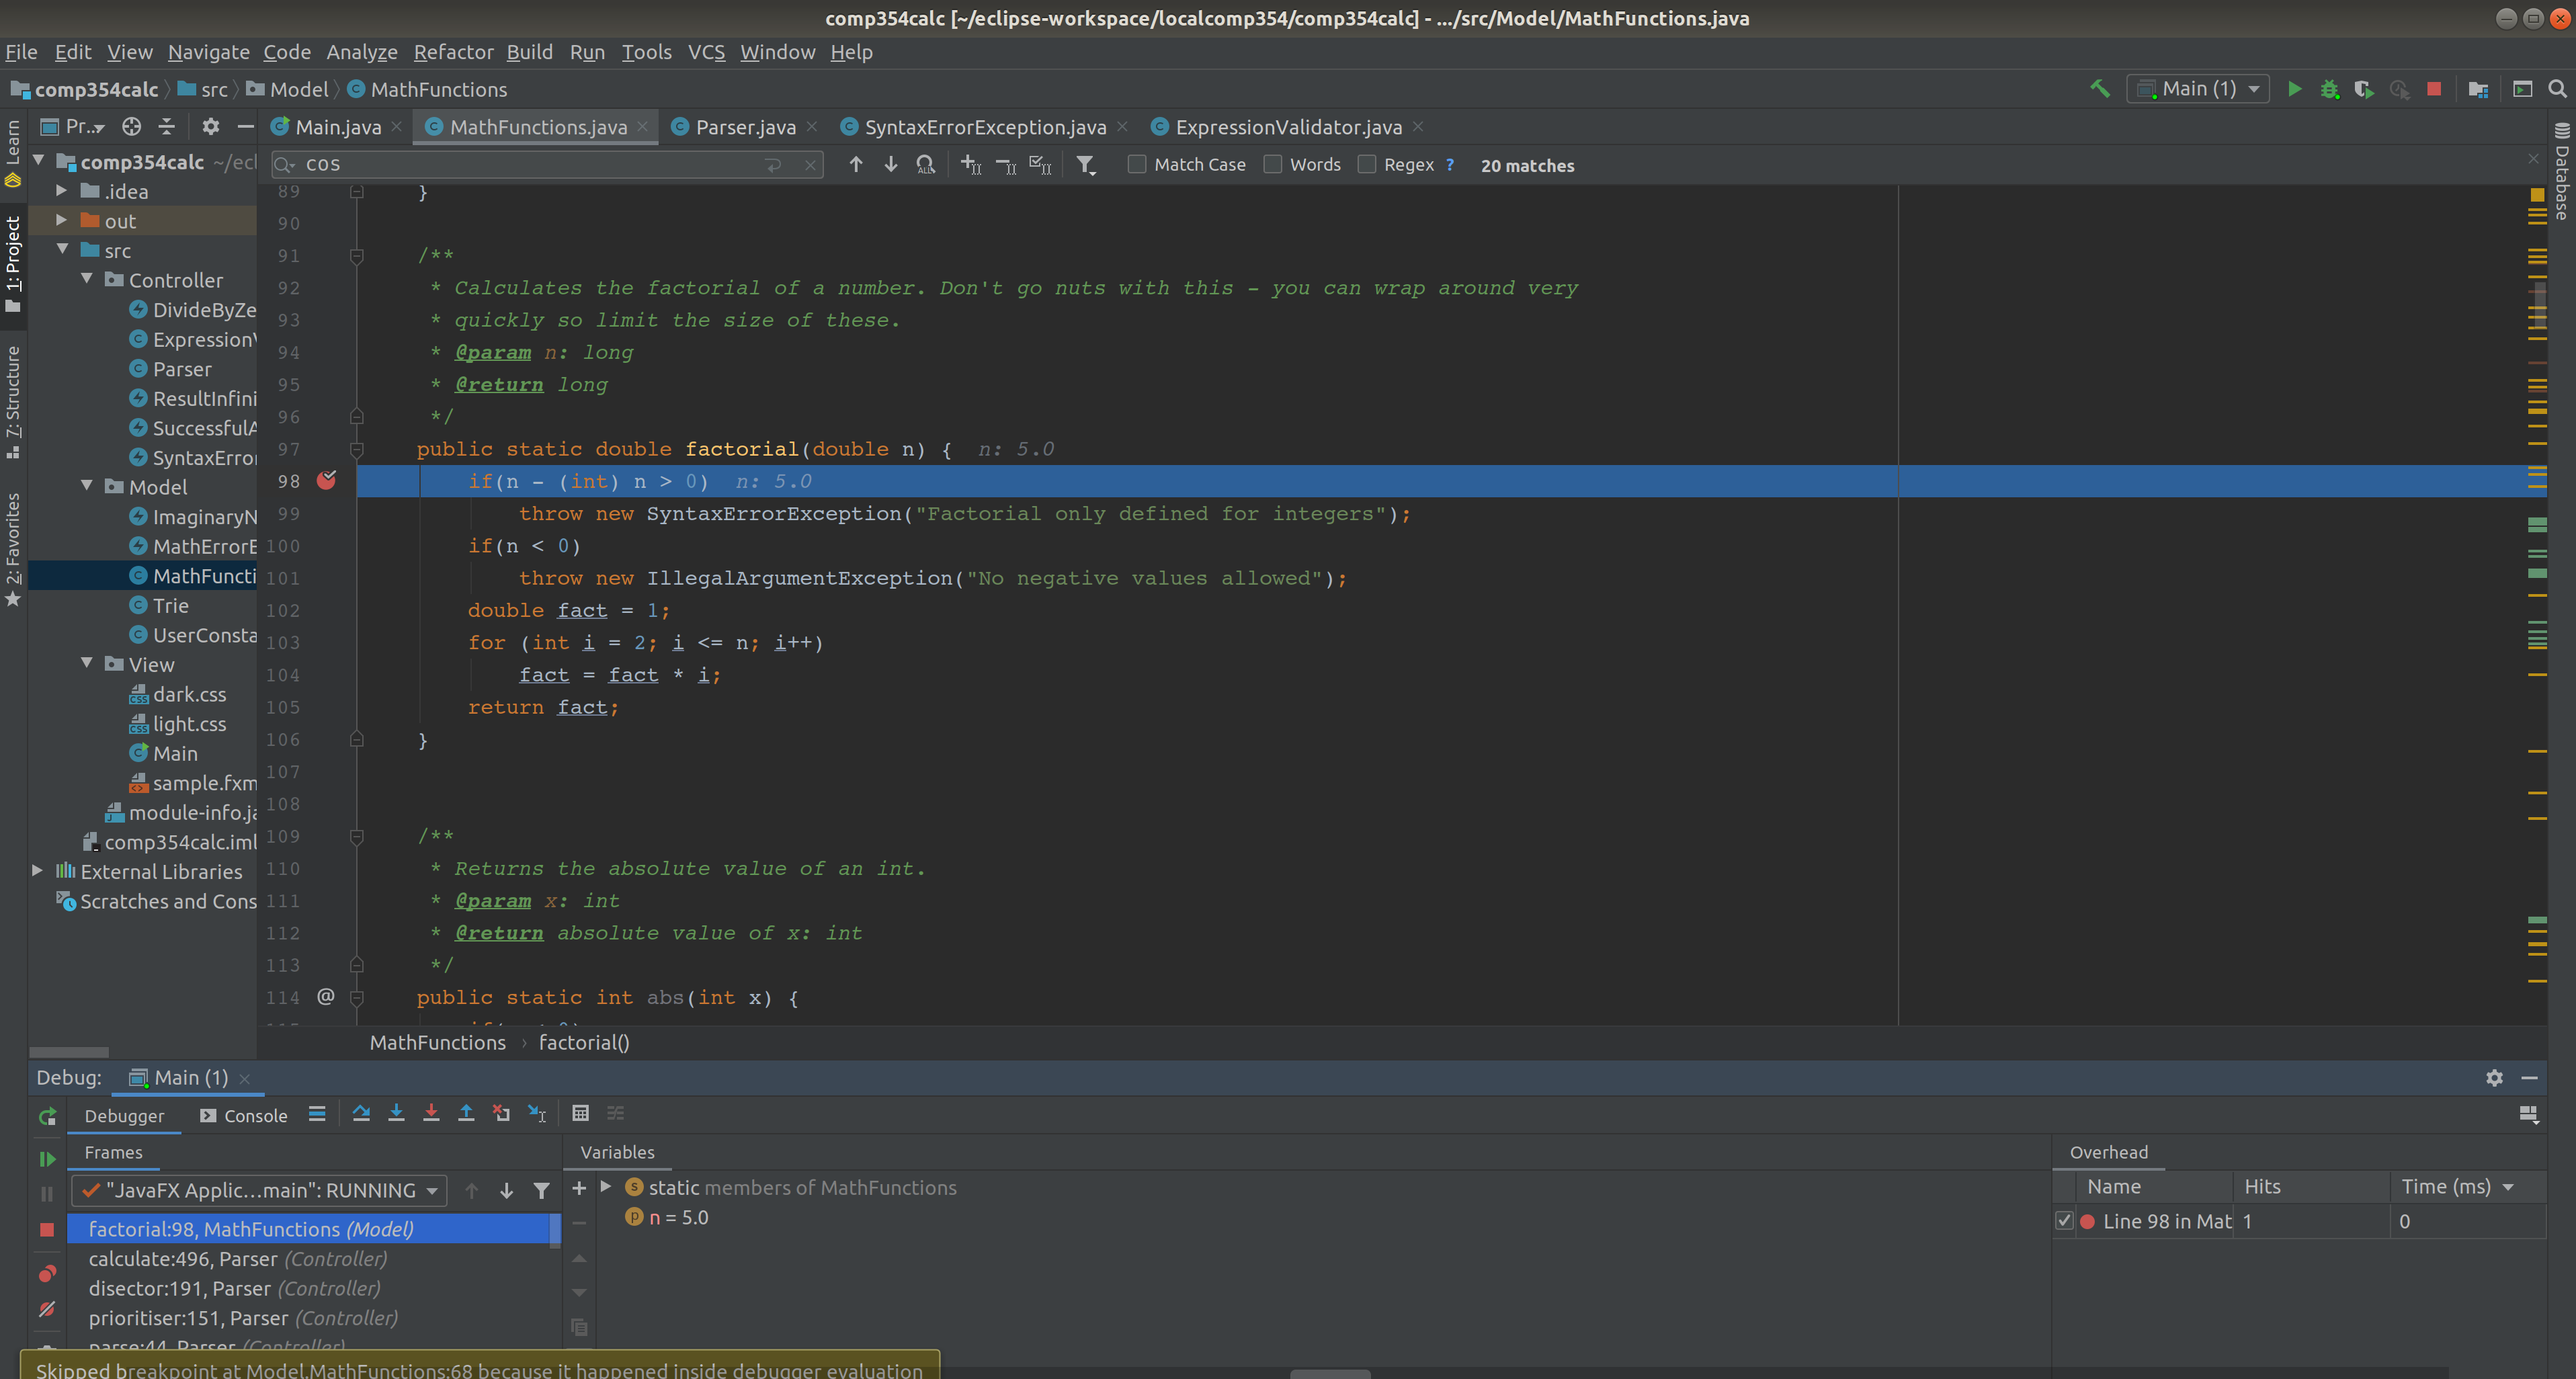
\includegraphics[width=1.13\textwidth]{Andres2.png}
\caption{Andres using the debugger to verify that the factorial function checks for integers}
\label{Andres2}
\end{figure}

\vspace{20mm}
\begin{figure}[H]
\centering
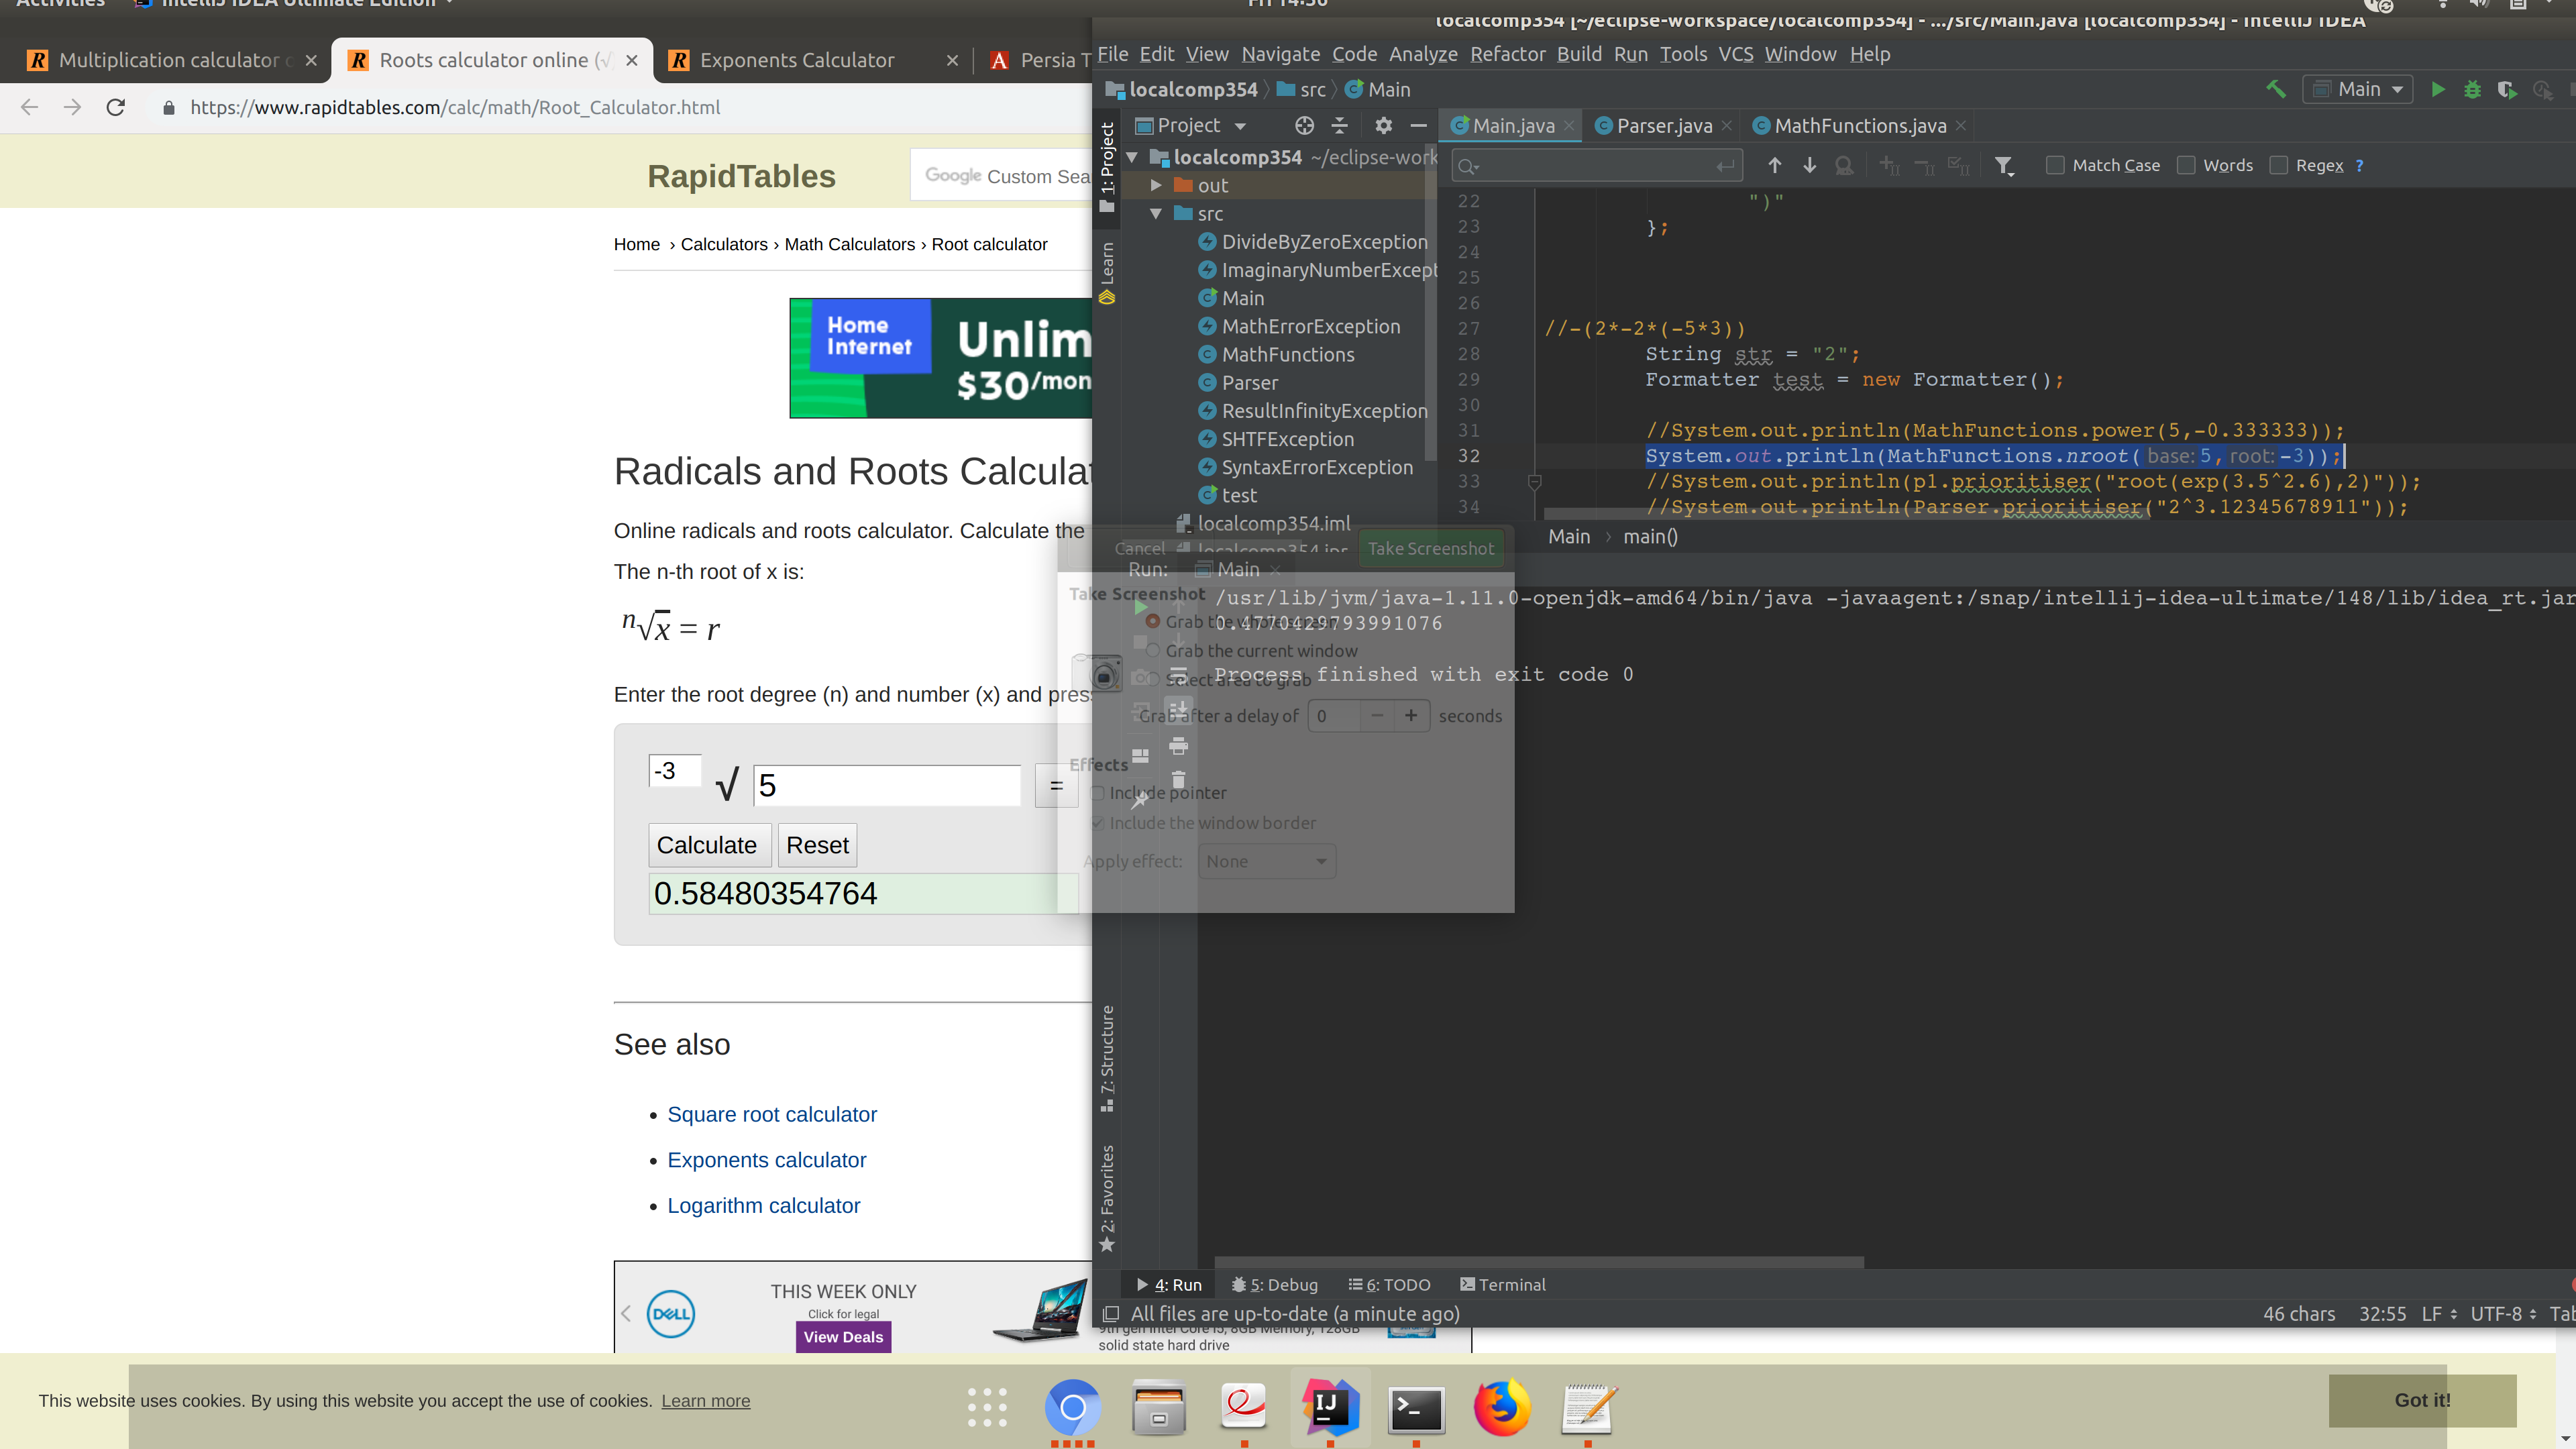
\includegraphics[width=1.13\textwidth]{Dany1.png}
\caption{Daniel F comparing the answer of our root function with the actual answer}
\label{Dany1}
\end{figure}

\vspace{20mm}
\begin{figure}[H]
\centering
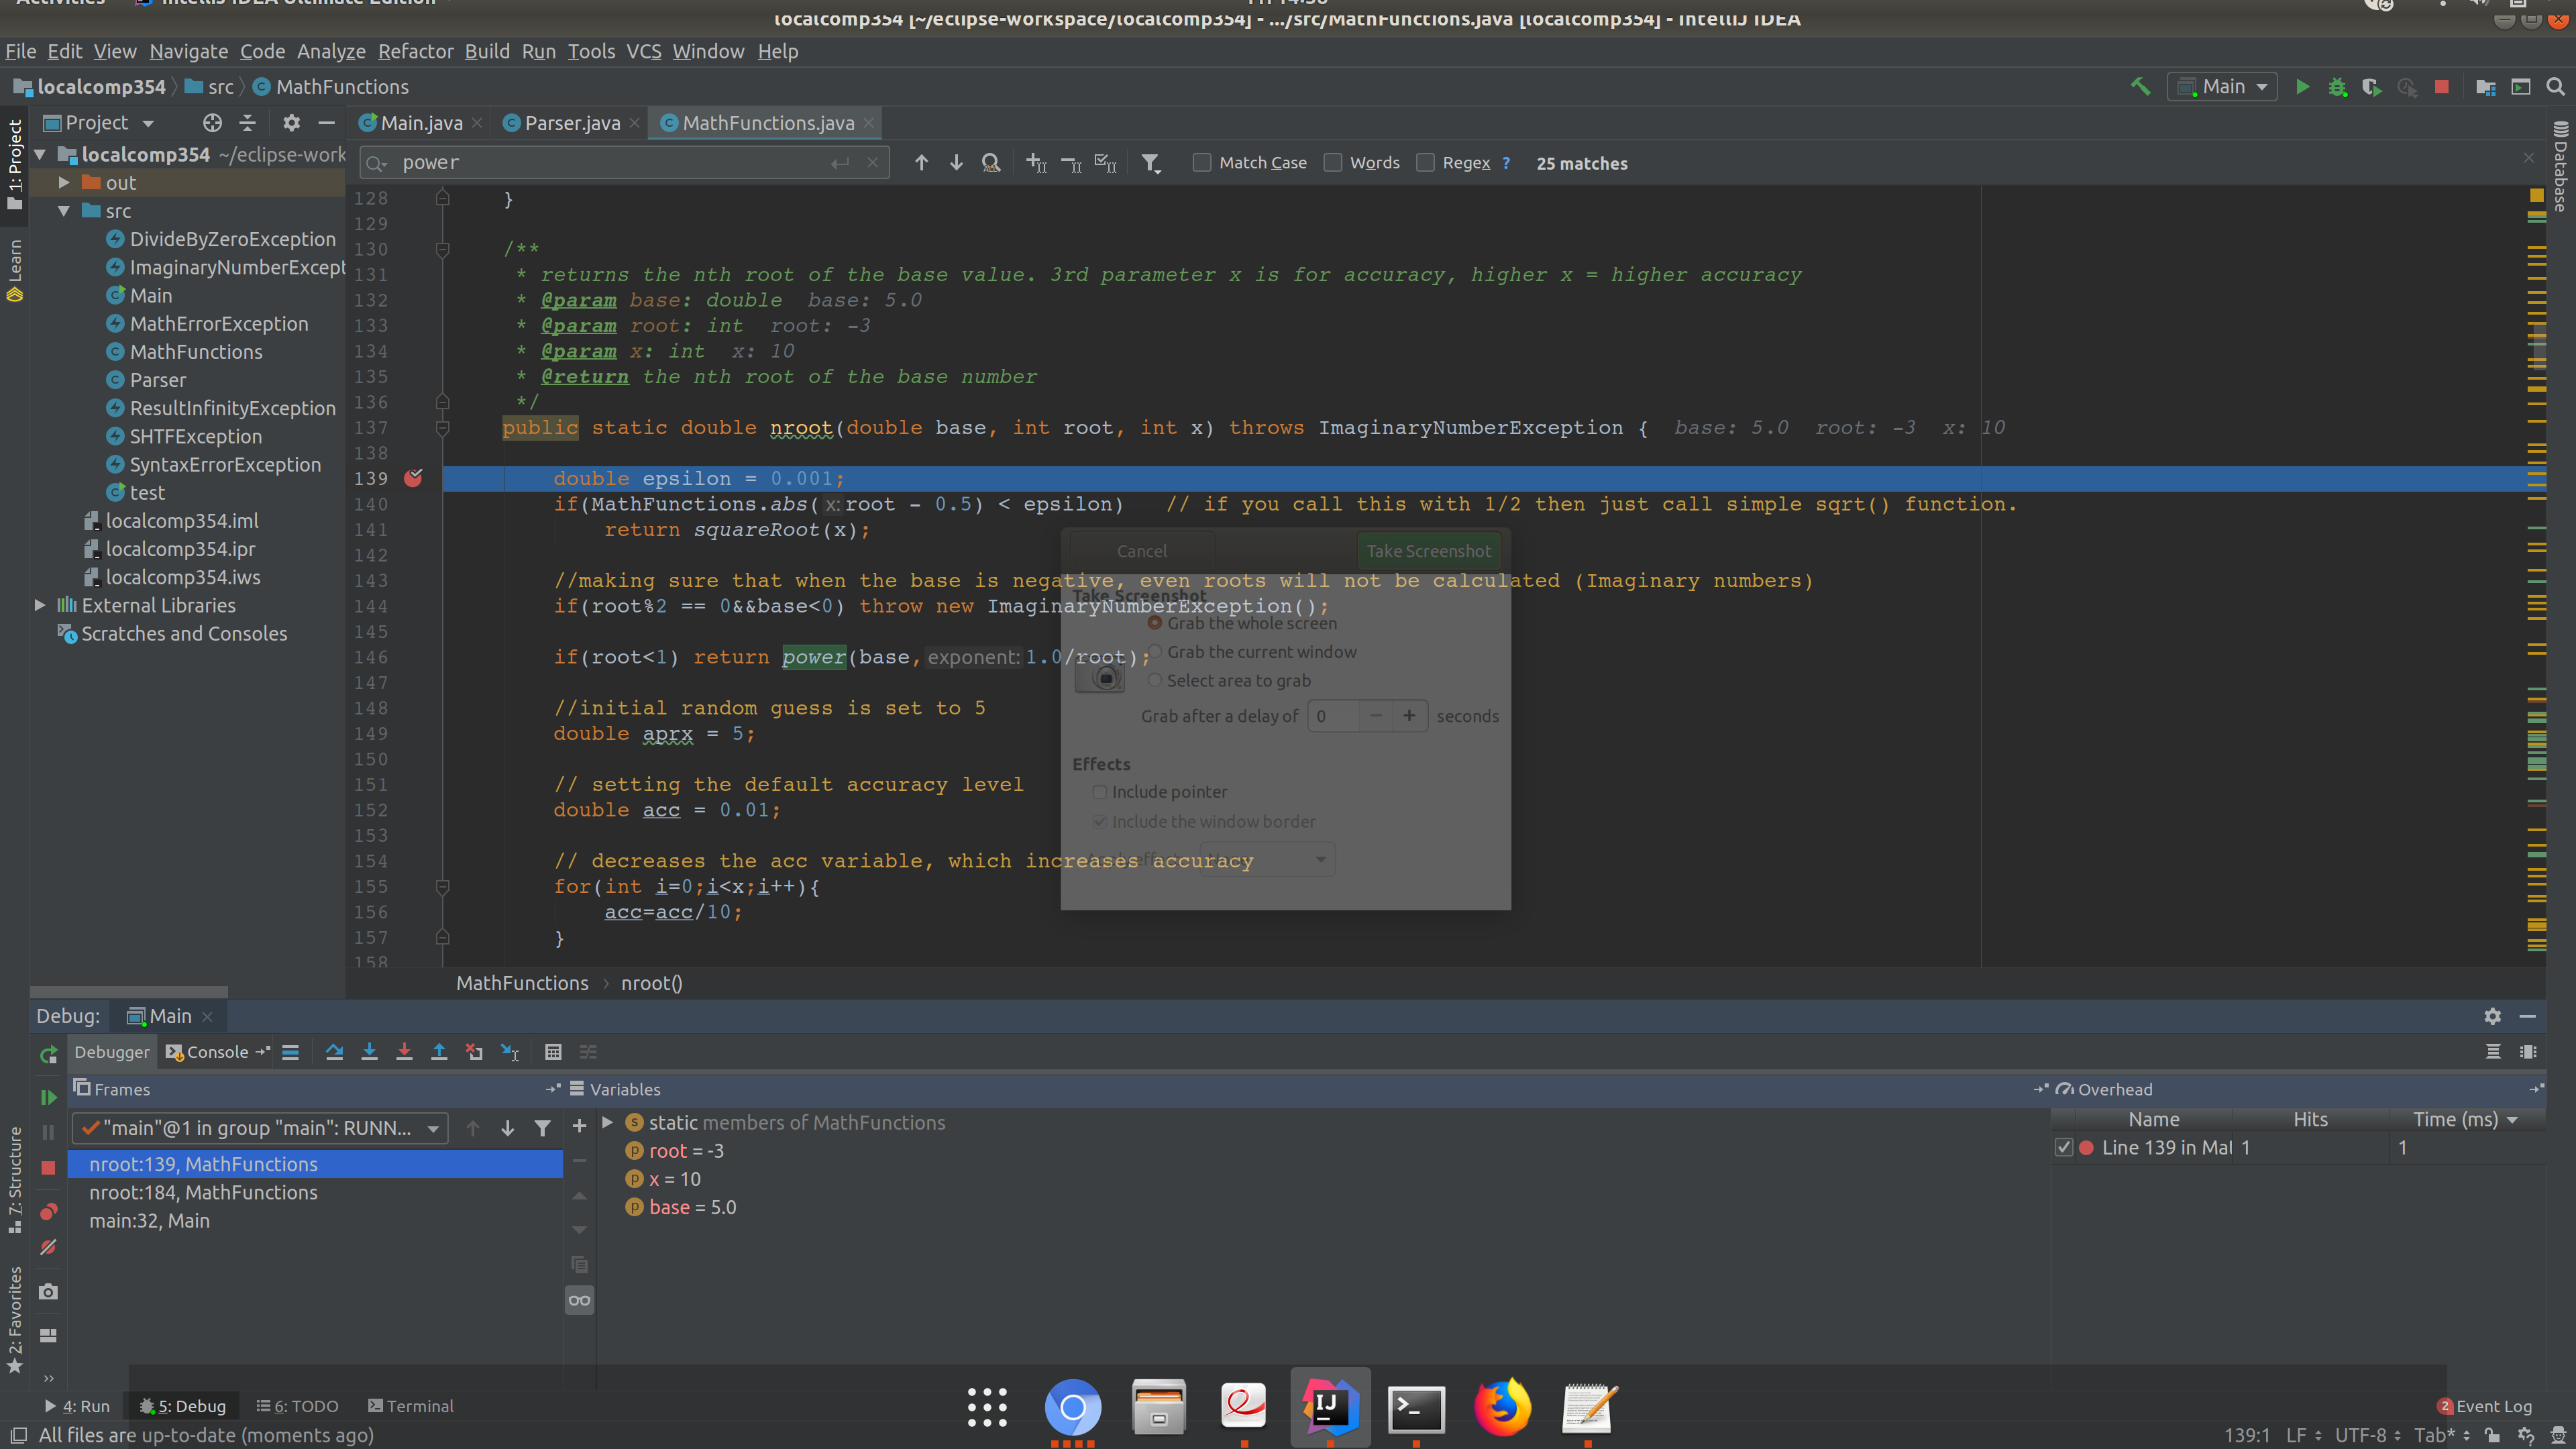
\includegraphics[width=1.13\textwidth]{Dany2.png}
\caption{Daniel F going through the root function to find why the answer is inaccurate }
\label{Dany2}
\end{figure}

\vspace{20mm}
\begin{figure}[H]
\centering
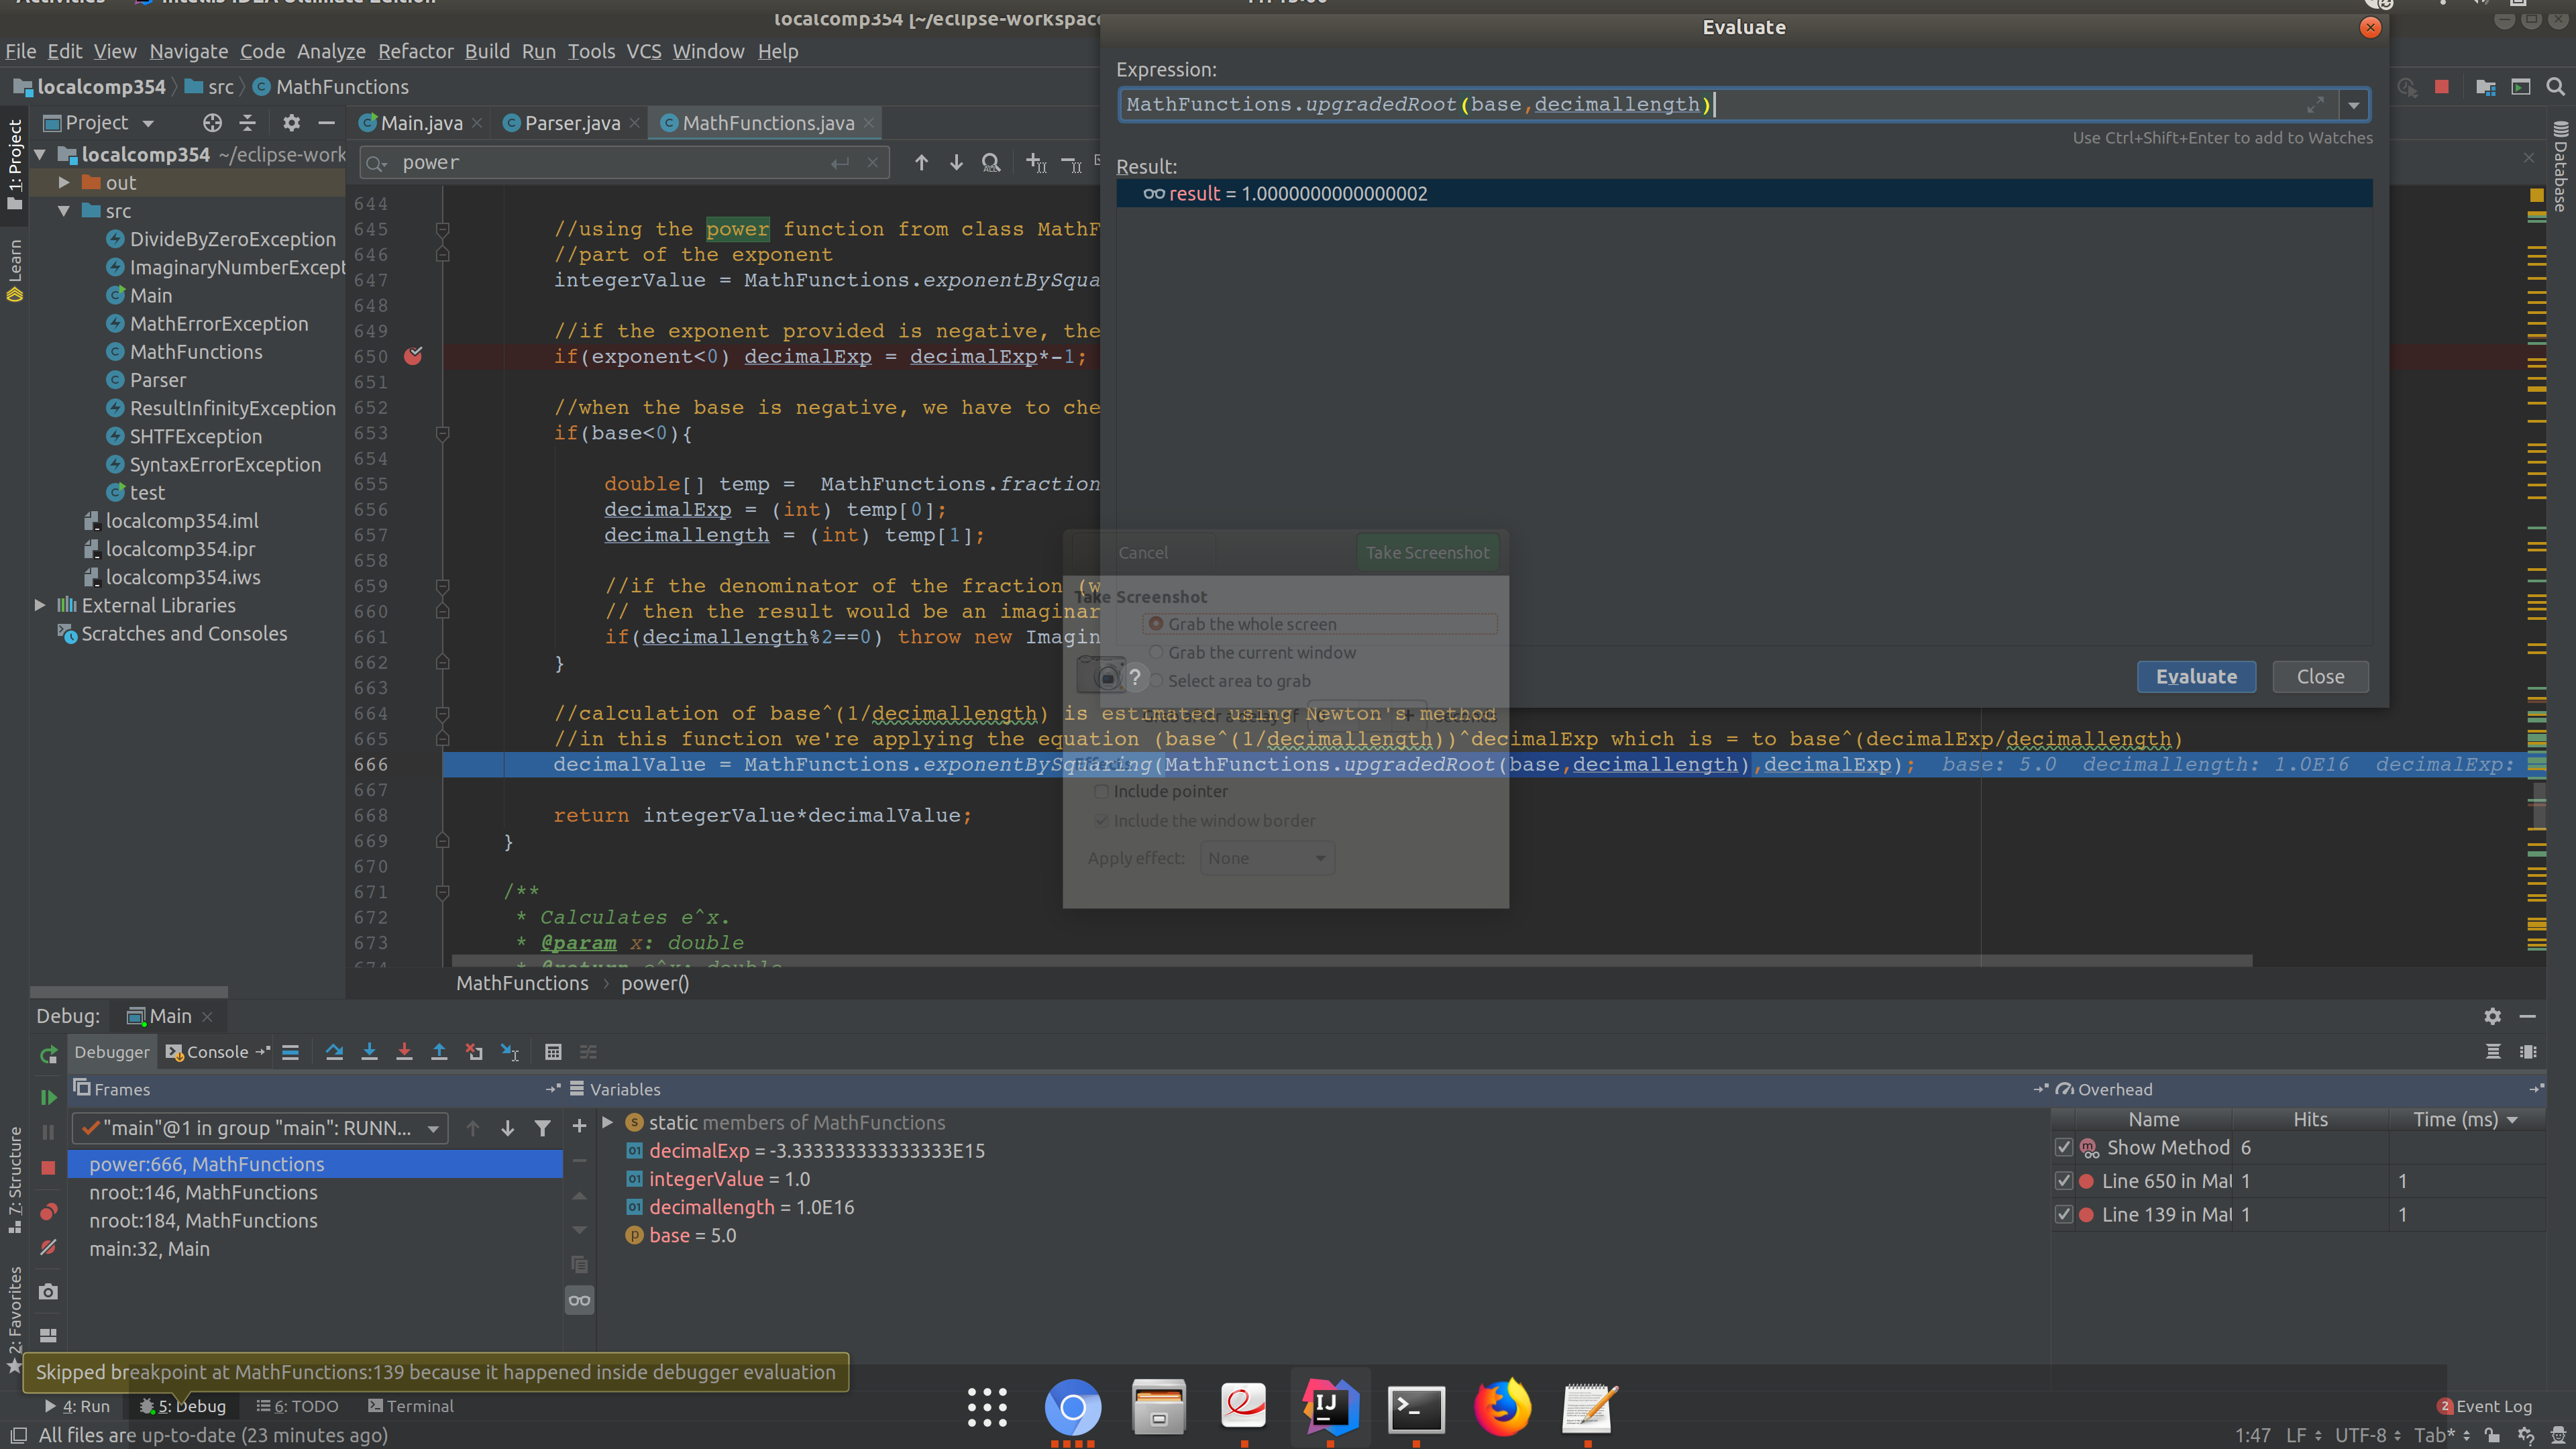
\includegraphics[width=1.13\textwidth]{Dany3.png}
\caption{Daniel F using the debugger to check why the power function is inaccurate}
\label{Dany3}
\end{figure}

\vspace{20mm}
\begin{figure}[H]
\centering
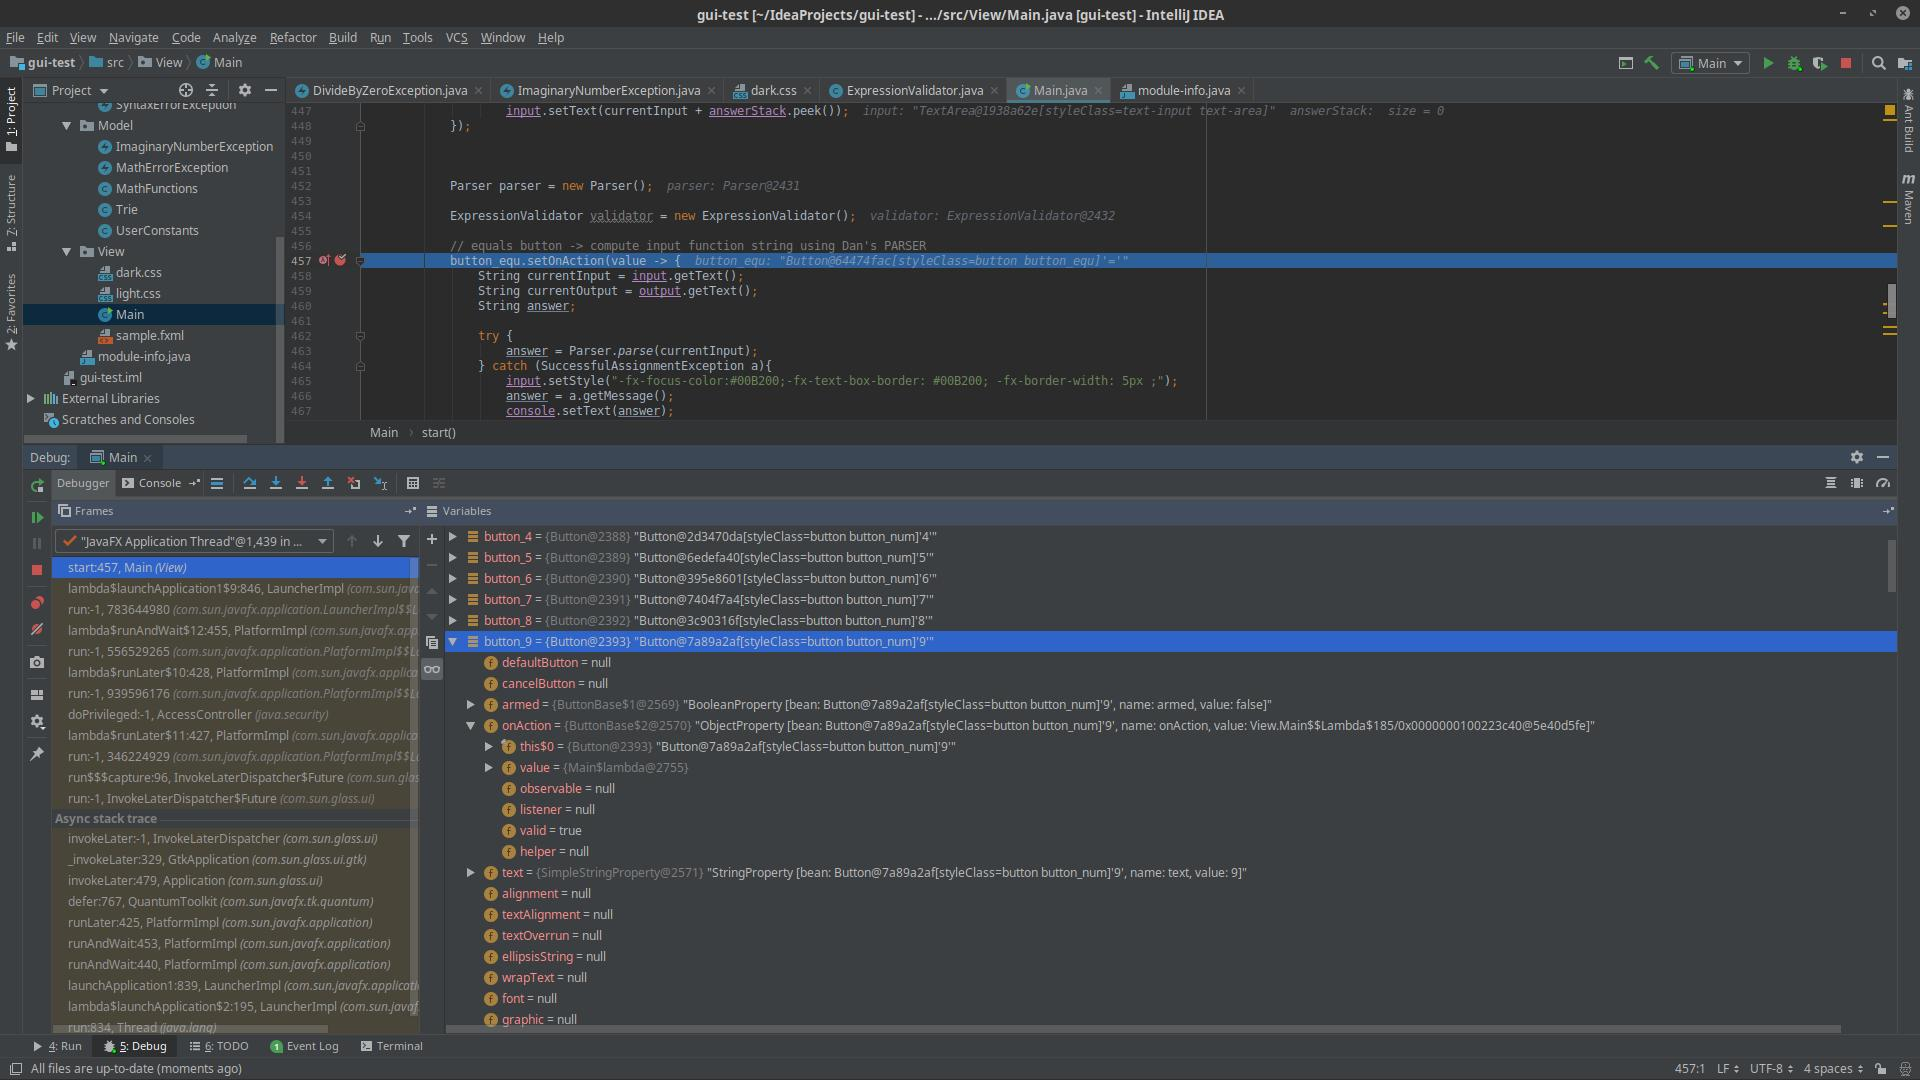
\includegraphics[width=1.13\textwidth]{justin.jpg}
\caption{Justin debugging a bug that caused a crash in the user interface}
\label{Justin}
\end{figure}


\vspace{20mm}
\begin{figure}[H]
\centering
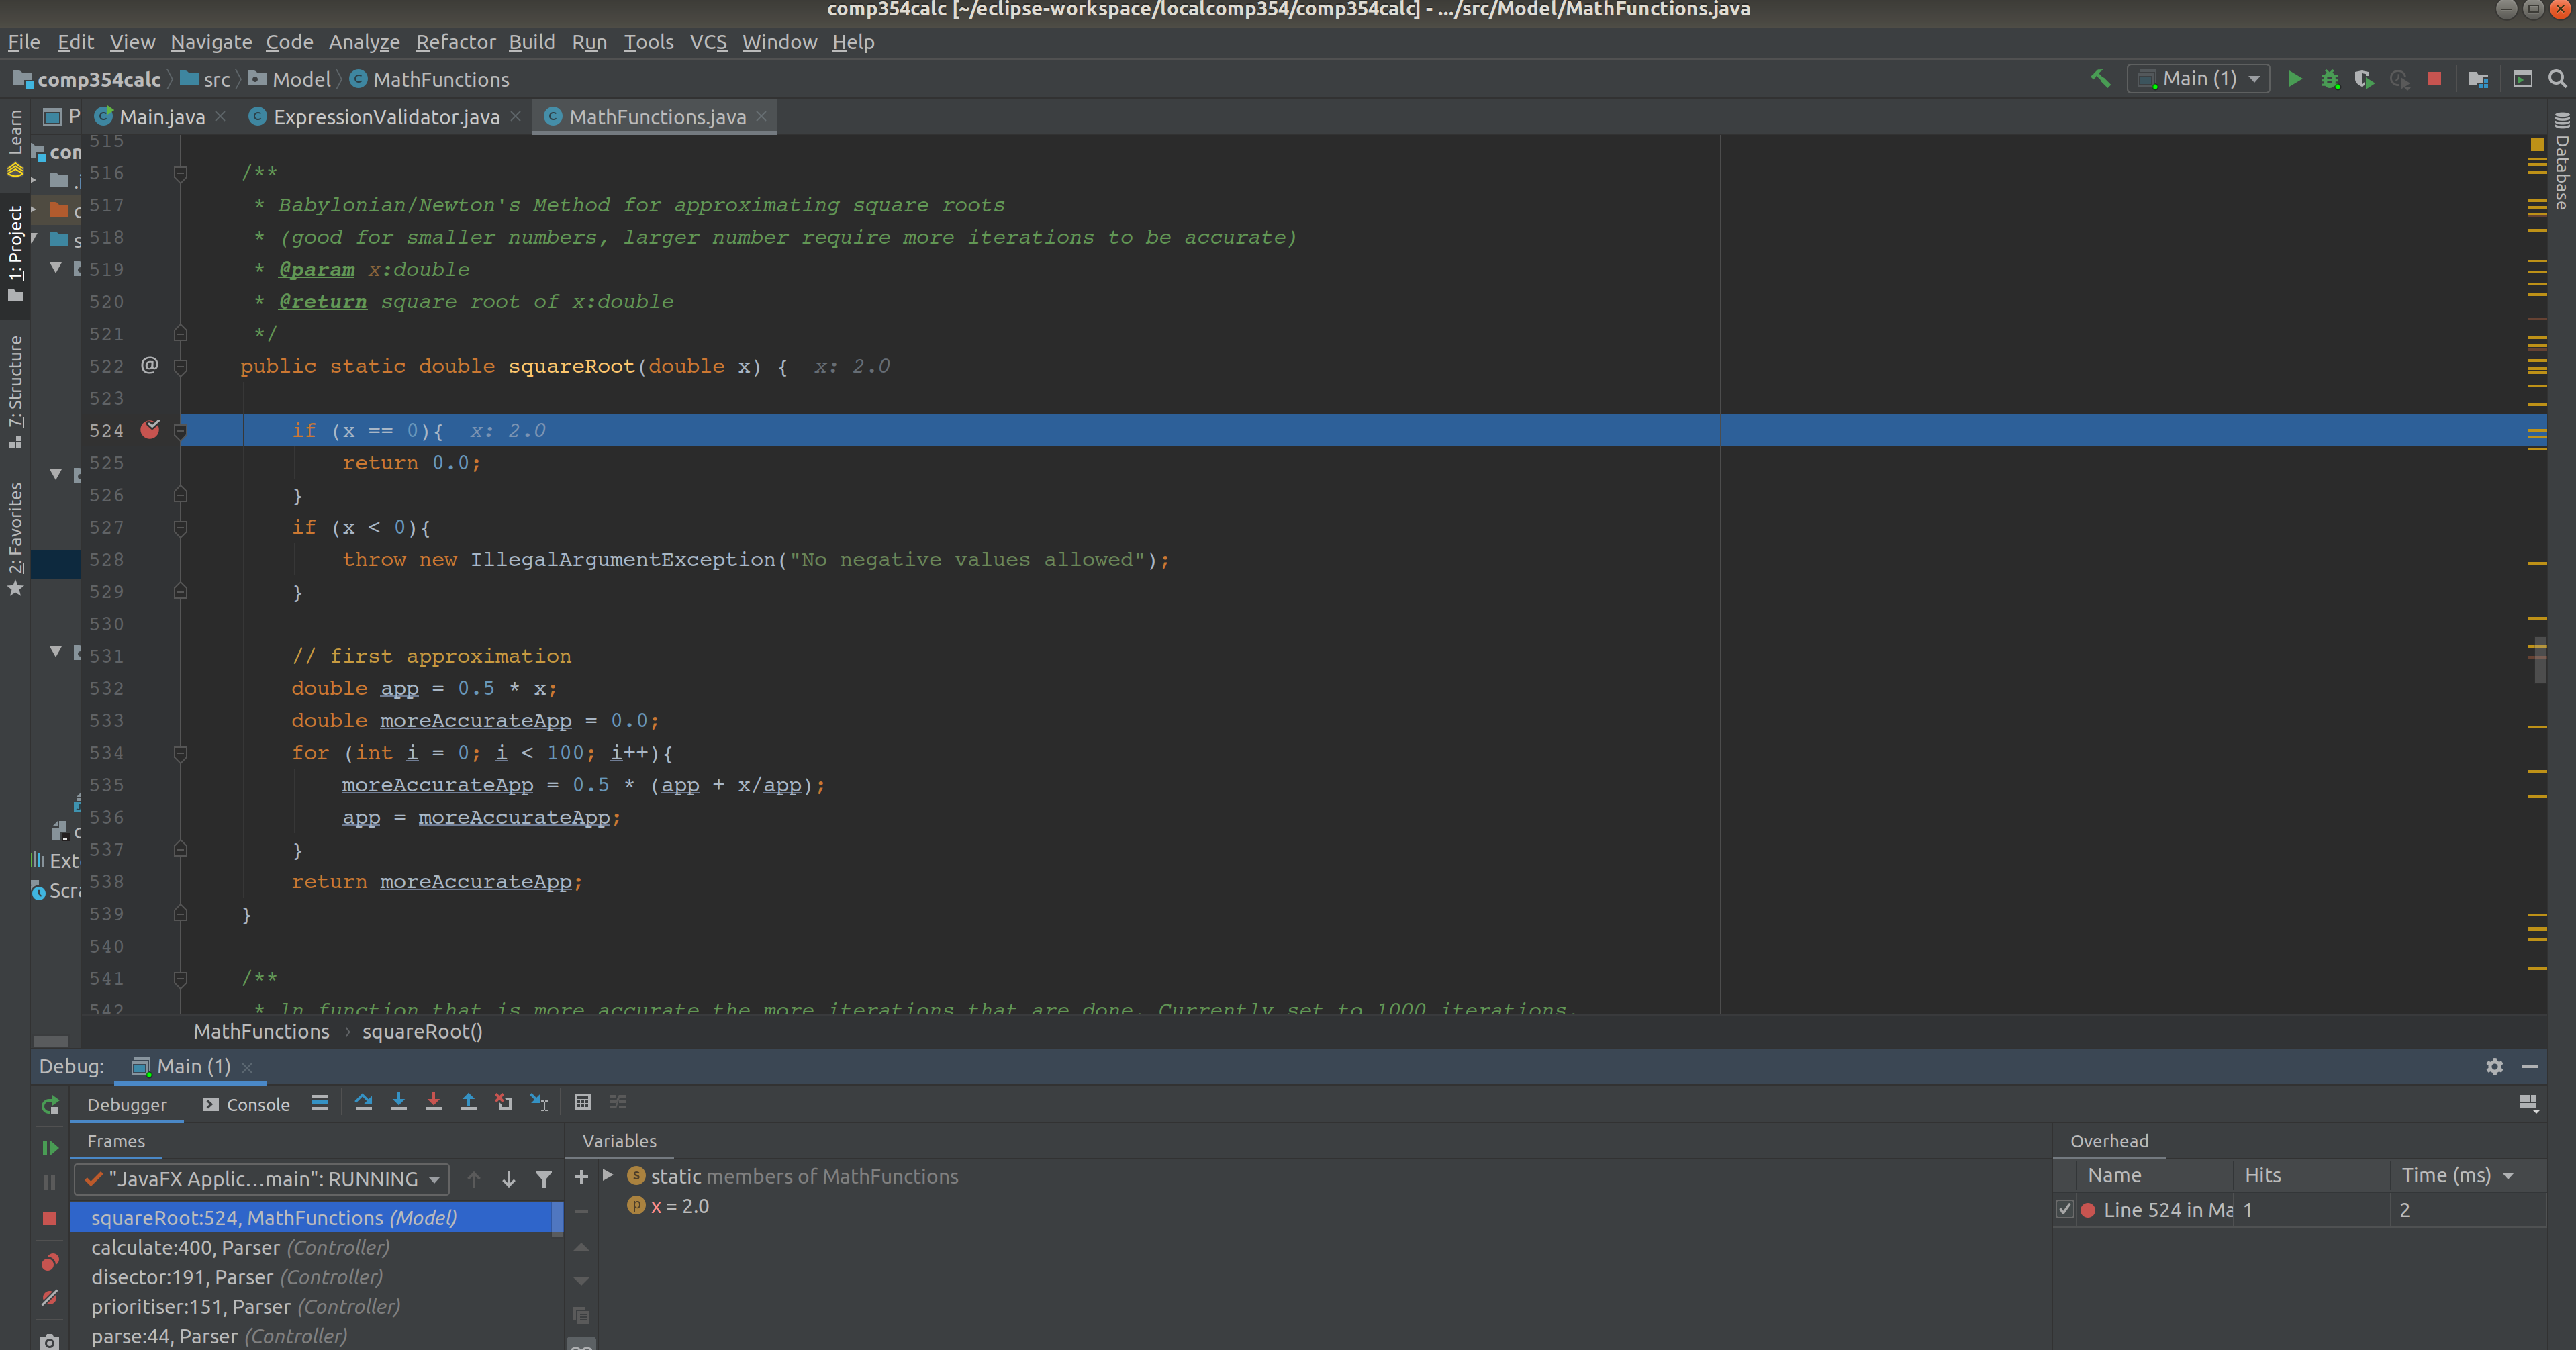
\includegraphics[width=1.13\textwidth]{Ashkan1.png}
\caption{Ashkan using the debugger to test find the bug in the square root function}
\label{Ashkan}
\end{figure}

\pagebreak

\subsection{Appendix B - ASQ Questions}

This section tests each of the functions below with real world problems in order to determine whether our Eternity calculator is reliable to use. We also used an online calculator frequently as reference to compare our calculator’s calculation precision/capability against it.
\\

The following are 5 word problems that can be solved using our calculator, using the following functions: 
\\

\begin{enumerate}
	\item $sin(x)$
	\item $e^(x)$
	\item $ln(x)$ 
	\item $x^y$ 
	\item $\sqrt{x}$
\end{enumerate}


\textbf{1) Word problem using Sin(x)}
\\

At 57" from the base of a building you need to look up at 55 degrees to see the top of a building. What is the height of the building? (Answer must be in the form of one decimal place)
\\

$tan(55)$ = $height/57$ 
\\

(Note:You must convert degrees to radians to solve problem. Input the degree value $x * \pi / 180$)
\\

55 degrees = 0.959931 radians

height = 57 * tan(55) = 81.4
\\

Ans: Our Eternity calculator result: $81.40443637404839 = 81.4$
\\

\textbf{2) Word problem that involves $e^x$ }
\\

Mitchell opened a savings account and deposited \$300.00 as principal. The account earns 13\% interest, compounded continuously. What is the balance after 1 year?
\\

Use the formula $A = Pert$, where A is the balance (final amount), P is the principal (starting amount), e is the base of natural logarithms ($\approx2.71828$), r is the interest rate expressed as a decimal, and t is the time in years.
\\

Round your answer to the nearest cent.
\\

Note:

Continuously compounded interest:
$A=Pert$

The variables in the equation are A, P, r, and t. The letter e is a constant.\\

A is the balance (final amount).\\
P is the principal (starting amount).\\
e is the base of natural logarithms.\\
r is the interest rate expressed as a decimal.\\
t is the time in years.\\
P=\$300.00, r=13\%=0.13, t=1 year\\

Now plug these values into the equation and solve for A.
Plug in $P = 300$, $r = 0.13$, and $t=1$
$= 300e0.13$
$\approx 341.648515$
$\approx \$341.65$
\\

Ans: Our Eternity calculator result: $341.6485149973866$ which is $341.65$ when rounded.
\\

\textbf{3) Logarithmic word problem ln(x)}
\\

The hydrogen ion concentration in a substance is [H+] = 0.98. We need to evaluate the pH at the given value of [H+]. Determine whether the substance is acidic or not (i.e. if the pH is less than 7).
\\

$pH = – log(H+) = – log(0.98)$
\\

\textbf{Ans:}

Online calculator result: $0.0087739243$

Our Eternity calculator result: $0.00877392430750515$

The pH is less than 7, so the substance is acidic.
\\

textbf{4) Power Function word problem $x^y$}
\\

Suppose a radioactive substance decays at a rate of 3.5\% per hour. What percent of the substance is left after 6 hours? 
\\

$100\%-5.5\% = 96.5\%$

$1-3.5 = 0.965$

$(0.965)^n x 100$

$(0.965)^6 x 100$
\\

\textbf{Ans:}

Online calculator result: $80.7539696082015625$

Our Eternity calculator result: $80.75396960820154$
\\

\textbf{5) Square root word problem $\sqrt{x}$}
\\

The area of a square screen is 100.35 cm2. Find the side length of the screen with an accuracy of 2 decimal places.
\\

$Area of square = (Side length) * 2$

$s = \sqrt{100.35}$
\\

\textbf{Ans:}

Online calculator result: $10.0174847142$

Our Eternity calculator result: $10.0174847142384$

\pagebreak

\subsection{Appendix C - Calculator Manual}

\begin{lstlisting}[language=TeX]


*Manual for Eternity Calculator :

*Description : Eternity Calculator is a calculator that 
               supports many mathematical functions while
               maintaining a simple and elegant look. Along 
               with its simple looks, Eternity has a range 
               of useful features, all of which will be 
               mentioned below.

*Requirements : 

    - Java 8 or lower

*Features : 

    (1) Support for Natural Language : (cos(2)^sqrt(2))

    (2) Assign constants : 
    - ex : a = 34
    - reserved letters : e (Eulers' number) , p (pi)
    - letters must be in lower case


    (2) Support for multiple themes (Dark/Light)

    (4) Error messages with feedback

(1) Supported Functions and Syntax 

    ( Capital words refer to user input )

      -Logarithm base 10 : log(N)

      -Logarithm with user defined base : log(B,N)

      -Linear logarithm : ln(N)

      -nth Root of a number: root(BASE,EXPONENT)

      -Square root : sqrt(N)

      -Cosine : cos(N)

      -Sine : sin(N)

      -Secant : sec(N)

      -Cosecant : csc(N)

      -Cotangent : cot(N)

      -e to the X : e^N

      -Power : N^X

      -Factorial : fact(N) Where N is an Integer

(2) Assigning constants 

      Alphabetical constants are assigned by typing a letter

      followed by an '=' sign and the value you wish to assign 

      to it.

      Note : (1) alphabetical constants must be in lower case

             (2) e and p are reserved characters fo Eulers' 

                 number and pi

(3) Changing Themes

      To changes theme, go to the Themes button in the top 

      menu bar, and select which theme you wish to use.

Author : 

      Written by Daniel Fakhr.

\end{lstlisting}

\pagebreak

\subsection{Appendix D - Macro Architecture Pattern (MVC)}

\begin{center}
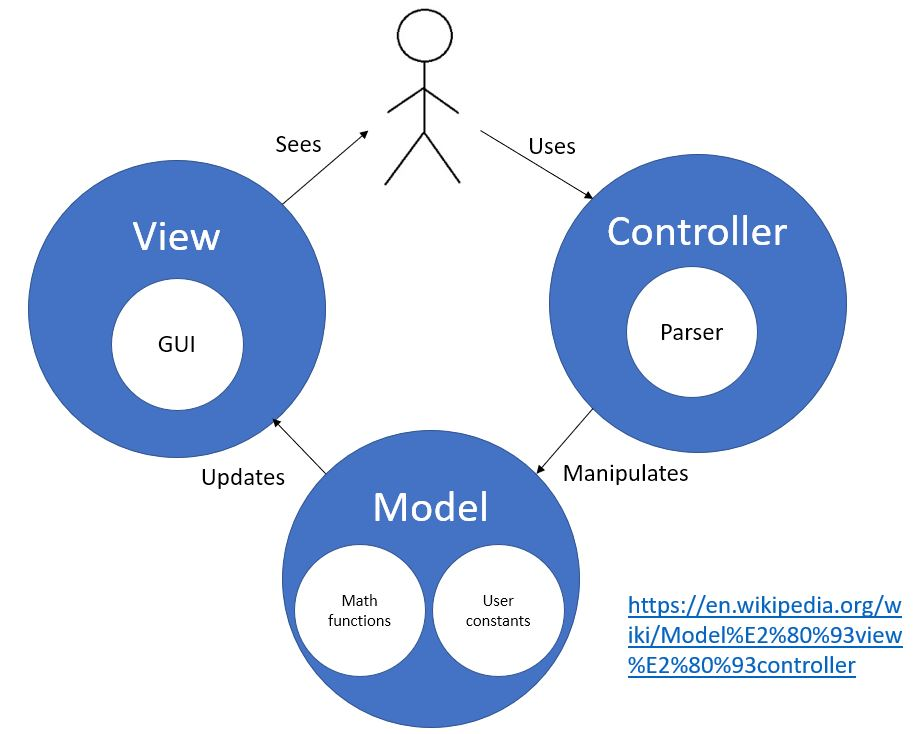
\includegraphics[width=0.9\textwidth]{Pattern.jpg}
\end{center}

\pagebreak

\subsection{Appendix E - Micro Architecture (MVC)}

\begin{center}
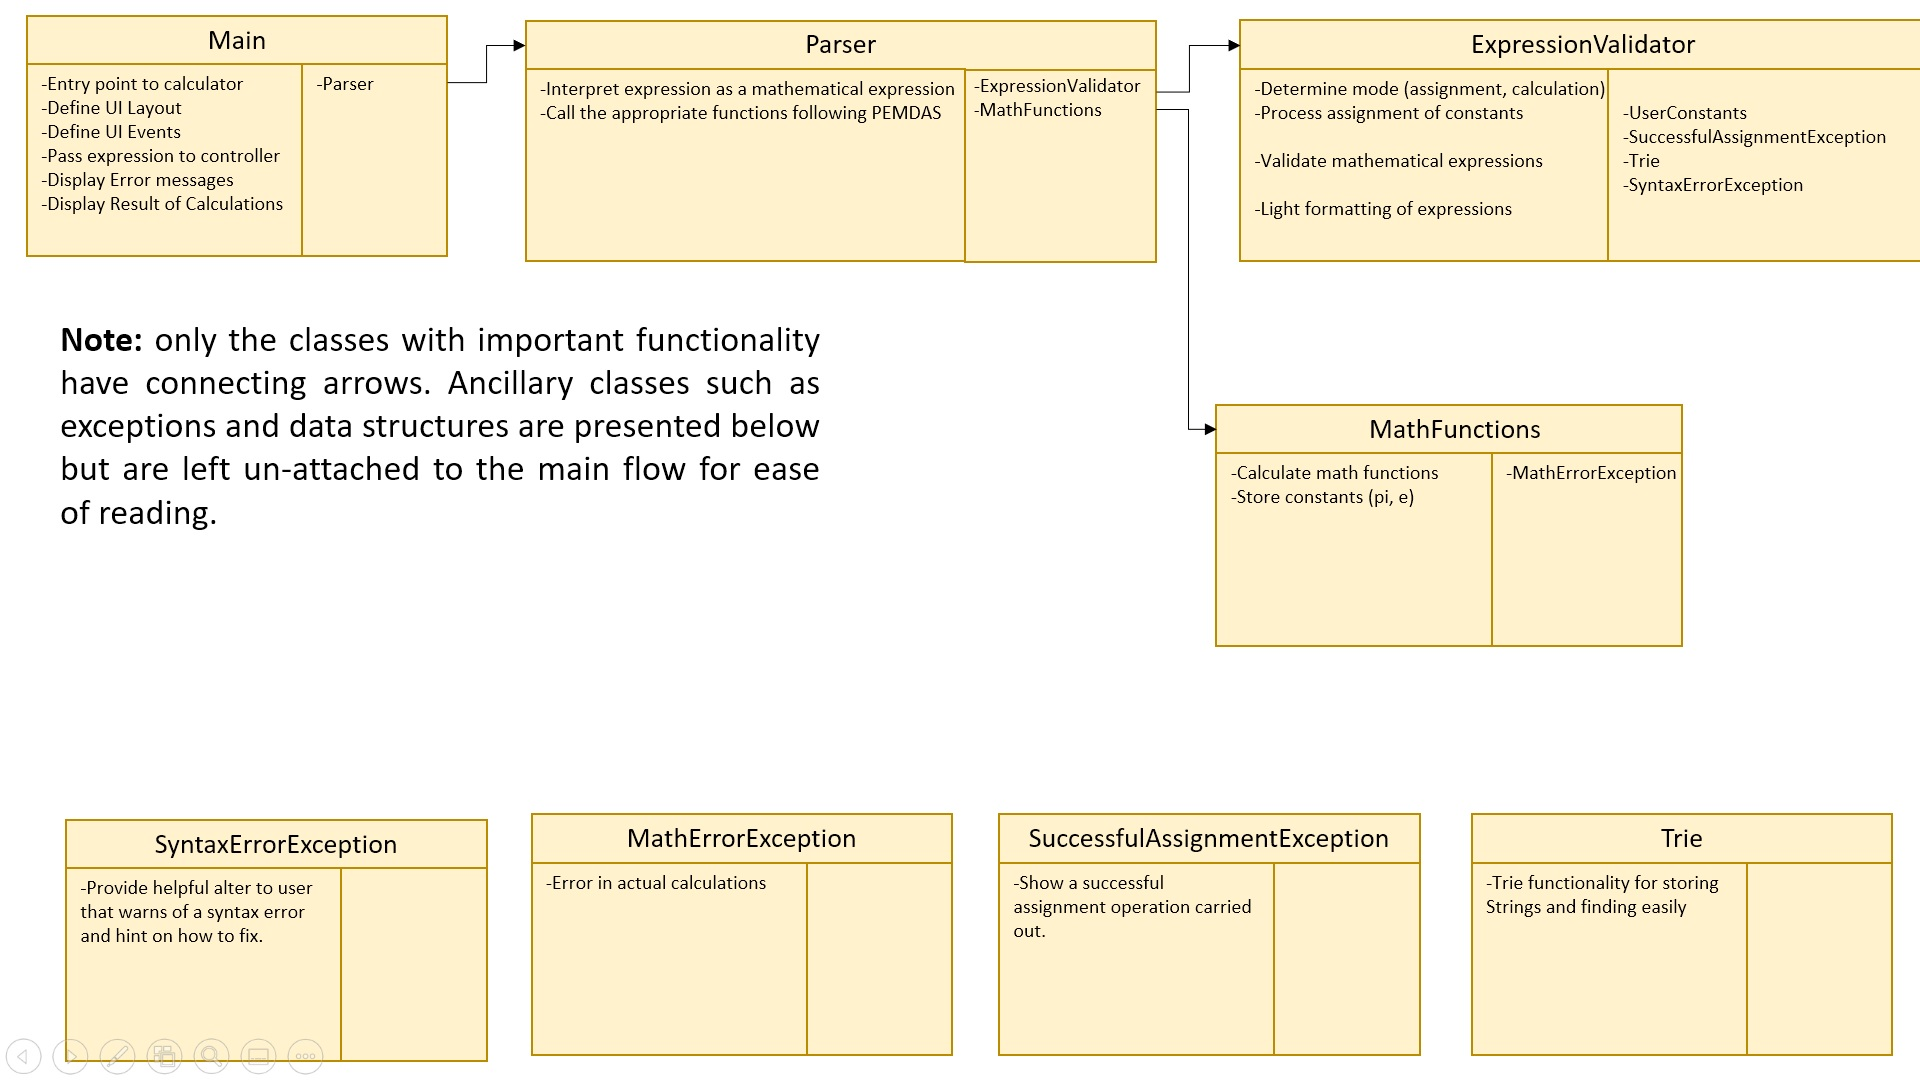
\includegraphics[angle=90,width=0.9\textwidth]{CRC.jpg}
\end{center}

\pagebreak



\subsection{Appendix E - Use Case Descriptions}

\begin{table}[!h]
\begin{tabular}{|p{3cm}|p{9cm}|}
\hline
\textbf{ID} & UC 1  \\ \hline
\textbf{Name} & Calculate result  \\ \hline
\textbf{Description} & User wants the calculator to resolve his mathematical expression to a satisfactory level of precision near-instantaneously.  \\ \hline
\textbf{Pre-condition} &
	\begin{itemize}
		\vspace{-2mm}
		\item Calculator is on
		\vspace{-3.5mm}
	\end{itemize}  \\ \hline
\textbf{Post-condition} &
	\begin{itemize}
		\vspace{-2mm}
		\item Calculator takes user input, parses, calculates, and arrives at a correct result.
		\item Calculator saves the result of this operation for future use (UC 2).
		\vspace{-3.5mm}
	\end{itemize}  \\ \hline
\textbf{Basic path} &
	\begin{enumerate}
		\vspace{-2mm}
		\item This use case starts with the user entering a mathematical expression into the calculator.
		\item When satisfied with inputted expression user presses "=" button or "enter" on keyboard.
		\item Calculator performs resolution of the arithmetic expression.
		\item Calculator stores the result of the expression (UC 4).
		\vspace{-3.5mm}
	\end{enumerate}  \\ \hline
\textbf{Alternative Path} &
	\begin{itemize}[leftmargin=6mm]
		\vspace{-2mm}
		\item [1b.] User enters a letter and number in order to store a variable (UC 3).
		\item [3a.] Calculator detects a syntax or arithmetic error in user's input.
			\begin{enumerate}
				\item Calculator detect the type of exception.
				\item Calculator displays this exception on screen (UC 4)
				\item User can clear exception and return to the offending arithmetic expression and attempt to correct the error (return to Basic Path 2).
			\end{enumerate}
		
		\vspace{-3.5mm}
	\end{itemize}  \\ \hline
\end{tabular}
\caption{UC 1 - Calculate result}
\end{table}
\pagebreak

\begin{table}[!h]
\begin{tabular}{|p{3cm}|p{9cm}|}
\hline
\textbf{ID} & UC 2  \\ \hline
\textbf{Name} & Recover previous result  \\ \hline
\textbf{Description} & User wants to recall the result of a previous calculation and be able use it in another calculation.  \\ \hline
\textbf{Pre-condition} &
	\begin{itemize}
		\vspace{-2mm}
		\item Calculator is on
		\item A successful calculation has already taken place (UC 1)
		\vspace{-3.5mm}
	\end{itemize}  \\ \hline
\textbf{Post-condition} &
	\begin{itemize}
		\vspace{-2mm}
		\item User sees result of previous calculation and can input it into another calculation.
		\vspace{-3.5mm}
	\end{itemize}  \\ \hline
\textbf{Basic path} &
	\begin{enumerate}
		\vspace{-2mm}
		\item User presses "Ans" button which will input result of the previous calculation into the current calculation.
		\item User carries on with the rest of the calculation (UC 1).
		\vspace{-3.5mm}
	\end{enumerate}  \\ \hline
\textbf{Alternative Path} &
	\begin{itemize}[leftmargin=6mm]
		\vspace{-2mm}
		\item [1a.] User can press "mem" button and see a list of previous results that can be chosen for the current calculation.
			\begin{enumerate}
				\item User presses "mem" button
				\item User scrolls to the desired result
				\item User presses "enter" button to insert select result into current calculation.
			\end{enumerate}
		
		\vspace{-3.5mm}
	\end{itemize}  \\ \hline
\end{tabular}
\caption{UC 2 - Recover previous result}
\end{table}
\pagebreak

\begin{table}[!h]
\begin{tabular}{|p{3cm}|p{9cm}|}
\hline
\textbf{ID} & UC 3  \\ \hline
\textbf{Name} & Store variables  \\ \hline
\textbf{Description} & User want to store values that can be recalled during calculations by referencing an alphabetical label.  \\ \hline
\textbf{Pre-condition} &
	\begin{itemize}
		\vspace{-2mm}
		\item Calculator is on
		\vspace{-3.5mm}
	\end{itemize}  \\ \hline
\textbf{Post-condition} &
	\begin{itemize}
		\vspace{-2mm}
		\item A number is stored in the calculator's memory and is ready to be retrieved by invoking its alphabetical label.
		\item User should be able to clear or overwrite a stored variable.
		\vspace{-3.5mm}
	\end{itemize}  \\ \hline
\textbf{Basic path} &
	\begin{enumerate}
		\vspace{-2mm}
		\item This use case starts with the user entering an alphabetical label that will eventually be used to recall the stored value.
		\item The user then presses "equals" to indicate that a value is to be stored under the chosen label.
		\item The user then presses "enter" which tells the calculator to store the variable under the aforementioned label.
		\item At any point during a calculation (UC 1), the user can evoke the value stored in a variable by entering the corresponding alphabetic character.
		\item The calculator substitutes the variables's value into the calculation.
		\vspace{-3.5mm}
	\end{enumerate}  \\ \hline
\textbf{Alternative Path} &
	\begin{itemize}[leftmargin=6mm]
		\vspace{-2mm}
		\item [1a.] Clearing the variable
			\begin{enumerate}
				\item User enters the alphabetic label of the variable that requires clearing (value and label appear on display).
				\item User presses "clear".
				\item The calculator shows the variable is now cleared.
			\end{enumerate}
		\vspace{-3.5mm}
	\end{itemize}  \\ \hline
\end{tabular}
\caption{UC 3 - Store variables}
\end{table}
\pagebreak

\begin{table}[!h]
\begin{tabular}{|p{3cm}|p{9cm}|}
\hline
\textbf{ID} & UC 4  \\ \hline
\textbf{Name} & Display Result  \\ \hline
\textbf{Description} & User wants clear display of the calculation as it is being inputted. User also wants the calculator to display clear results and appropriate error messages. \\ \hline
\textbf{Pre-condition} &
	\begin{itemize}
		\vspace{-2mm}
		\item Result was calculated, or
		\item User inputs values in calculator
		\vspace{-3.5mm}
	\end{itemize}  \\ \hline
\textbf{Post-condition} & 
	\begin{itemize}
		\vspace{-2mm}
		\item Intermediate calculation is displayed on screen.
		\item Final results are displayed on screen.
		\item Error messages are displayes correctly.
		\vspace{-3.5mm}
	\end{itemize}  \\ \hline
\textbf{Basic path} &
	\begin{enumerate}
		\vspace{-2mm}
		\item User turns on the calculator
			\begin{itemize}
			\item [1a.] Welcome message is displayed.
			\end{itemize}
		\item User enters a calculation. The input calculation is displayed on scree as it is typed.
		\item User presses "=" to calculate (UC 1).
		\item The result of the calculation is displayed on screen.
		\vspace{-3.5mm}
	\end{enumerate}  \\ \hline
\textbf{Alternative Path} &
	\begin{itemize}[leftmargin=6mm]
		\vspace{-2mm}
		\item [4a.] An error occured and the appropriate message is displayed to the user.
			\begin{itemize}
			\item [1] User can clear the error and attempt to correct it.
			\end{itemize}
		
		\vspace{-3.5mm}
	\end{itemize}  \\ \hline
\end{tabular}
\caption{UC 4 - Calculate result}
\end{table}

\pagebreak


\end{document}

